\section{Search Methodology}

\subsection{Initial Search Conditions}
Searching for the best parameters requires defining the conditions that the chosen parameter set must satisfy. Consequently, those conditions must rely on metrics that depend on the parameters. We use the following:

\begin{itemize}
    \item \textbf{Size}: the size of the signature in bytes (B);
    \item \textbf{KeyGen}: the number of SHA-256 compressions ($C$) to generate a key pair;
    \item \textbf{SigGen}: the number of compressions to sign a message;
    \item \textbf{SigVer}: the number of compressions to verify a signature;
    \item \textbf{$\rho$}: SigVer per signature byte, in $C$/B.
\end{itemize}

We choose SLH-DSA-128s as the baseline for the search; this gives us an intuitive way to compare custom parameter sets against the standardized scheme on equal footing.

Costs count SHA-256 compressions with the $\mathsf{PK.seed}$ block compressed once per key pair, as FIPS~205 allows and the SHRINCS reference implementation does; Appendix~\ref{app:hash-convention} details this convention and gives the SLH-DSA-128s costs under it.

\subsection{Toolset}
The methodology described here uses a set of SageMath scripts available at \url{https://github.com/BlockstreamResearch/SPHINCS-Parameters}.

All figures and tables in this report are generated by the accompanying pipeline (\texttt{make generate}). An interactive explorer that reproduces these searches — including the filter coefficients, decisional weights, and distance criteria used in this report — is publicly available at \url{https://blockstreamresearch.github.io/SPHINCS-Parameters/site/}.

\subsection{Sweep Strategy} \label{sec:sweep-strategy}
We start by enumerating all parameter tuples $(h, d, k, a, w)$. Applying the initial bounds (security level, size $\leq$ SLH-DSA, at least $2^{40}$ supported signatures) reduces the search space from \emph{34,580} candidates to \emph{7,570} — a $78\%$ cut. The remaining space is still too large to inspect by hand, so we need additional filters.

We introduce the following filters\footnote{The coefficient for each filter, except the signature size, may be greater than 1 (meaning we accept some regression on that metric in exchange for gains elsewhere).}:

\begin{itemize}
    \item \textbf{Bound on size}: $\mathsf{target.size} \leq c_{\text{size}} \cdot \mathsf{std.size}$, where $c_{\text{size}}$ is a size coefficient ($0 \leq c_{\text{size}} \leq 1$).
    \item \textbf{Bound on KeyGen}: $\mathsf{target.KeyGen} \leq c_{\text{kg}} \cdot \mathsf{std.KeyGen}$, where $c_{\text{kg}} > 0$.
    \item \textbf{Bound on SigGen}: $\mathsf{target.SigGen} \leq c_{\text{sg}} \cdot \mathsf{std.SigGen}$, where $c_{\text{sg}} > 0$.
    \item \textbf{Bound on SigVer}: $\mathsf{target.SigVer} \leq c_{\text{sv}} \cdot \mathsf{std.SigVer}$, where $c_{\text{sv}} > 0$.
    \item \textbf{Bound on $\rho$}: $\mathsf{target}.\rho \leq c_{\text{cb}} \cdot \mathsf{std}.\rho$, where $c_{\text{cb}} > 0$.
\end{itemize}

Verification and signing costs are averages over uniformly random messages; Appendix~\ref{app:average-case} compares them with the worst case.


These filters can be combined and parameterized in different ways to produce different result sets. Below, we consider several cases to illustrate how the choice of filter parameters affects the resulting candidate set.

\subsubsection{Case 1: Best in Class}
In this case, we find the most efficient signature for a single metric at a time, leaving the other metrics unbounded. The results are shown in Table~\ref{tab:minimal_metric_each}.

\begin{table}[h!]
\small
\raggedright 
\caption{Absolute Global Extremes}
\label{tab:minimal_metric_each}
\resizebox{\textwidth}{!}{%
\begin{tabular}{llrrrrrrrrr}
\toprule
\textbf{Award Category} & \textbf{Tuple $(h, d, k, a, w)$} & \textbf{Size (B)} & \textbf{VS std, \%} & \textbf{KeyGen ($C$)} & \textbf{VS std, $\times$} & \textbf{SigGen ($C$)} & \textbf{VS std, $\times$} & \textbf{SigVer ($C$)} & \textbf{VS std, $\times$} & \textbf{$\rho$ ($C$/B)} \\
\midrule
%---
\texttt{STANDARD} Baseline & $(63, 7, 14, 12, 16)$ & $7856$ & $+0.0\%$ & $2.92 \times 10^5$ & $1.00$ & $2.22 \times 10^6$ & $1.00$ & $2193$ & $1.00$ & $0.28$ \\
%---
Smallest Signature & $(50, 2, 6, 20, 256)$ & \textcolor{green}{$3408$} & \textcolor{green}{$-56.6\%$} & \textcolor{red}{$1.55 \times 10^{11}$} & \textcolor{red}{$5.30 \times 10^5$} & \textcolor{red}{$3.10 \times 10^{11}$} & \textcolor{red}{$1.40 \times 10^5$} & \textcolor{red}{$5022$} & \textcolor{red}{$2.29$} & \textcolor{red}{$1.47$} \\
%---
Fastest KeyGen & $(40, 8, 7, 20, 16)$ & \textcolor{red}{$7488$} & \textcolor{red}{$-4.7\%$} & \textcolor{green}{$1.83 \times 10^4$} & \textcolor{green}{$0.06$} & \textcolor{red}{$2.22 \times 10^7$} & \textcolor{red}{$9.99$} & \textcolor{orange}{$2411$} & \textcolor{orange}{$1.10$} & \textcolor{orange}{$0.32$} \\
%---
Fastest SigGen & $(42, 7, 20, 8, 16)$ & \textcolor{red}{$7488$} & \textcolor{red}{$-4.7\%$} & \textcolor{green}{$3.65 \times 10^4$} & \textcolor{green}{$0.12$} & \textcolor{green}{$2.71 \times 10^5$} & \textcolor{green}{$0.12$} & \textcolor{orange}{$2172$} & \textcolor{orange}{$0.99$} & \textcolor{orange}{$0.29$} \\
%---
Fastest SigVer & $(50, 2, 6, 20, 2)$ & \textcolor{red}{$7184$} & \textcolor{red}{$-8.6\%$} & \textcolor{red}{$1.03 \times 10^{10}$} & \textcolor{red}{$3.54 \times 10^4$} & \textcolor{red}{$2.07 \times 10^{10}$} & \textcolor{red}{$9.33 \times 10^3$} & \textcolor{green}{$389$} & \textcolor{green}{$0.18$} & \textcolor{green}{$0.05$} \\
%---
Lowest $\rho$ & $(50, 2, 6, 20, 2)$ & \textcolor{red}{$7184$} & \textcolor{red}{$-8.6\%$} & \textcolor{red}{$1.03 \times 10^{10}$} & \textcolor{red}{$3.54 \times 10^4$} & \textcolor{red}{$2.07 \times 10^{10}$} & \textcolor{red}{$9.33 \times 10^3$} & \textcolor{green}{$389$} & \textcolor{green}{$0.18$} & \textcolor{green}{$0.05$} \\
\bottomrule
\end{tabular}%
}
\end{table}


Table~\ref{tab:minimal_metric_each} confirms what one would suspect: each metric can be minimized impressively in isolation, but only at a brutal cost to the others, leaving these parameter sets unusable in practice. We therefore consider a different strategy.

\subsubsection{Case 2: Balanced Metrics}
In the next experiment, we look for ``average'' candidates whose metrics all stay below a uniform threshold $X \cdot \mathsf{std}$ (the filter is applied to every metric, with the exception of the maximum signature size $\leq \mathsf{std}$). By gradually increasing $X$, we obtain the following picture.
\begin{figure}[h!]
    \centering
    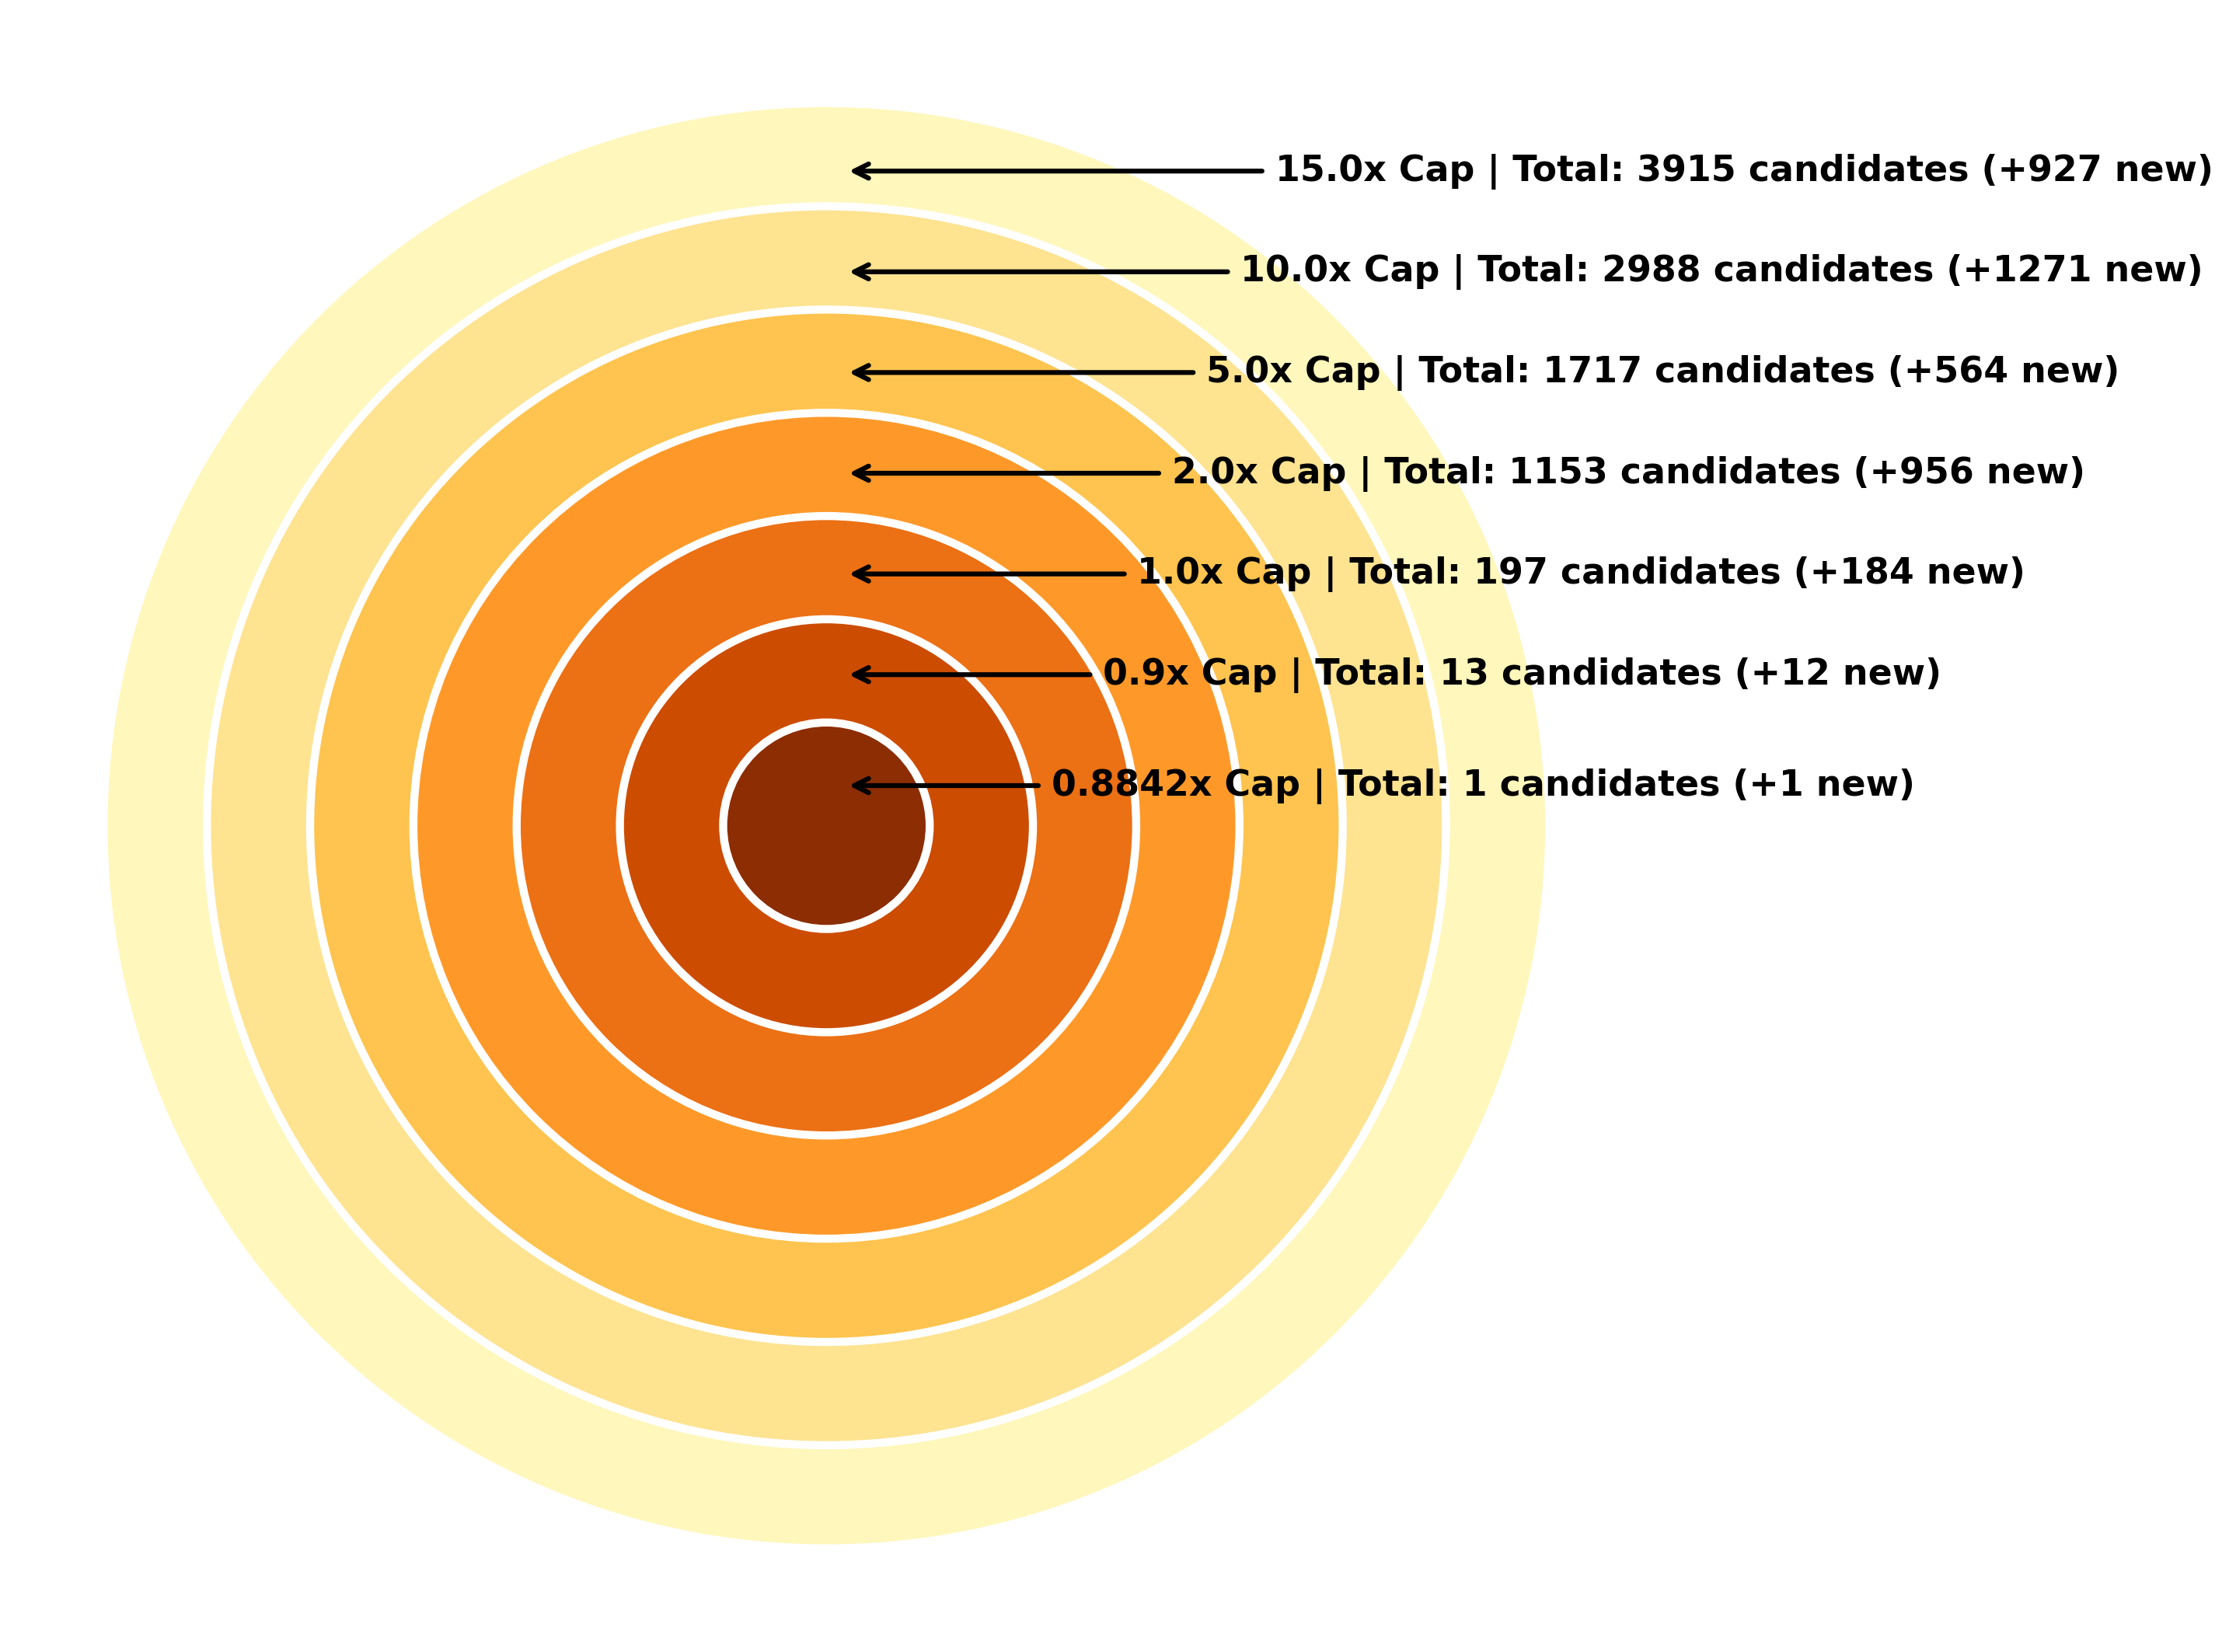
\includegraphics[width=0.8\textwidth]{content/images/concentric_diagram.png}
    \caption{Global Minimax Expansion: Concentric Euler diagram illustrating the volume of candidates unlocked at expanding uniform multiplier thresholds.}
    \label{fig:concentric_minimax}
\end{figure}

Naturally, the smaller the multiplier $X$, the fewer candidates survive the filter. A clear winner emerges at $X \approx 0.8666$; let us see how compelling it actually is (Table~\ref{tab:optimal_candidate_metrics}).

\begin{table}[h!]
    \centering
\small
\caption{Performance Comparison between the Standard Baseline and the Balanced Candidate}
\label{tab:optimal_candidate_metrics}
\begin{tabular}{lrrr}
\toprule
\textbf{Metric} & \textbf{Standard Baseline} & \textbf{Optimal Candidate} & \textbf{Ratio} \\
\midrule
        Parameters $(h, d, k, a, w)$ & $(63, 7, 14, 12, 16)$ & $(40, 5, 19, 10, 16)$ & -- \\
        Size (B) & $7{,}856$ & $6{,}800$ & $0.8656\times$ \\
        KeyGen ($C$) & $292{,}351$ & $146{,}175$ & $0.5000\times$ \\
        SigGen ($C$) & $2{,}218{,}486$ & $789{,}237$ & $0.3558\times$ \\
        SigVer ($C$) & $2{,}193$ & $1{,}645$ & $0.7501\times$ \\
        $\rho$ ($C$/B) & $0.2791$ & $0.2419$ & $0.8666\times$ \\
\bottomrule
\end{tabular}
\end{table}

One might call this a reasonable result. We are less impressed: a 13\% saving on signature size is not particularly attractive on its own (the goal is to materially close the gap with Schnorr).

\subsubsection{Case 3: Adaptive Search}
The strategy is straightforward:
\begin{enumerate}
    \item Decide which sacrifices you are willing to make on each metric.
    \item Find the best candidate among those that remain.
\end{enumerate}

For step (1) we apply the filters introduced in Section~\ref{sec:sweep-strategy}. This subsection is dedicated to step (2).

Each candidate is uniquely defined by its tuple of metric values, so the search for an optimal candidate can be cast as finding the point closest to the origin in a five-dimensional space (analogous to a shortest-vector problem, but mercifully confined to a small set of survivors), where each axis represents one of our metrics. That is almost the whole story.

To build intuition, suppose we care about only two metrics — signature size and signature generation cost. We require the signature size to be no larger than that of SLH-DSA, and we are willing to tolerate a signing cost of at most $2\times$ the standard. In this case all admissible candidates fit inside the green rectangle in Figure~\ref{fig:scatter_plot}, which makes brute-force inspection easy: the best candidate is simply the point closest to the origin $(0, 0)$.

\begin{figure}[h!]
    \centering
    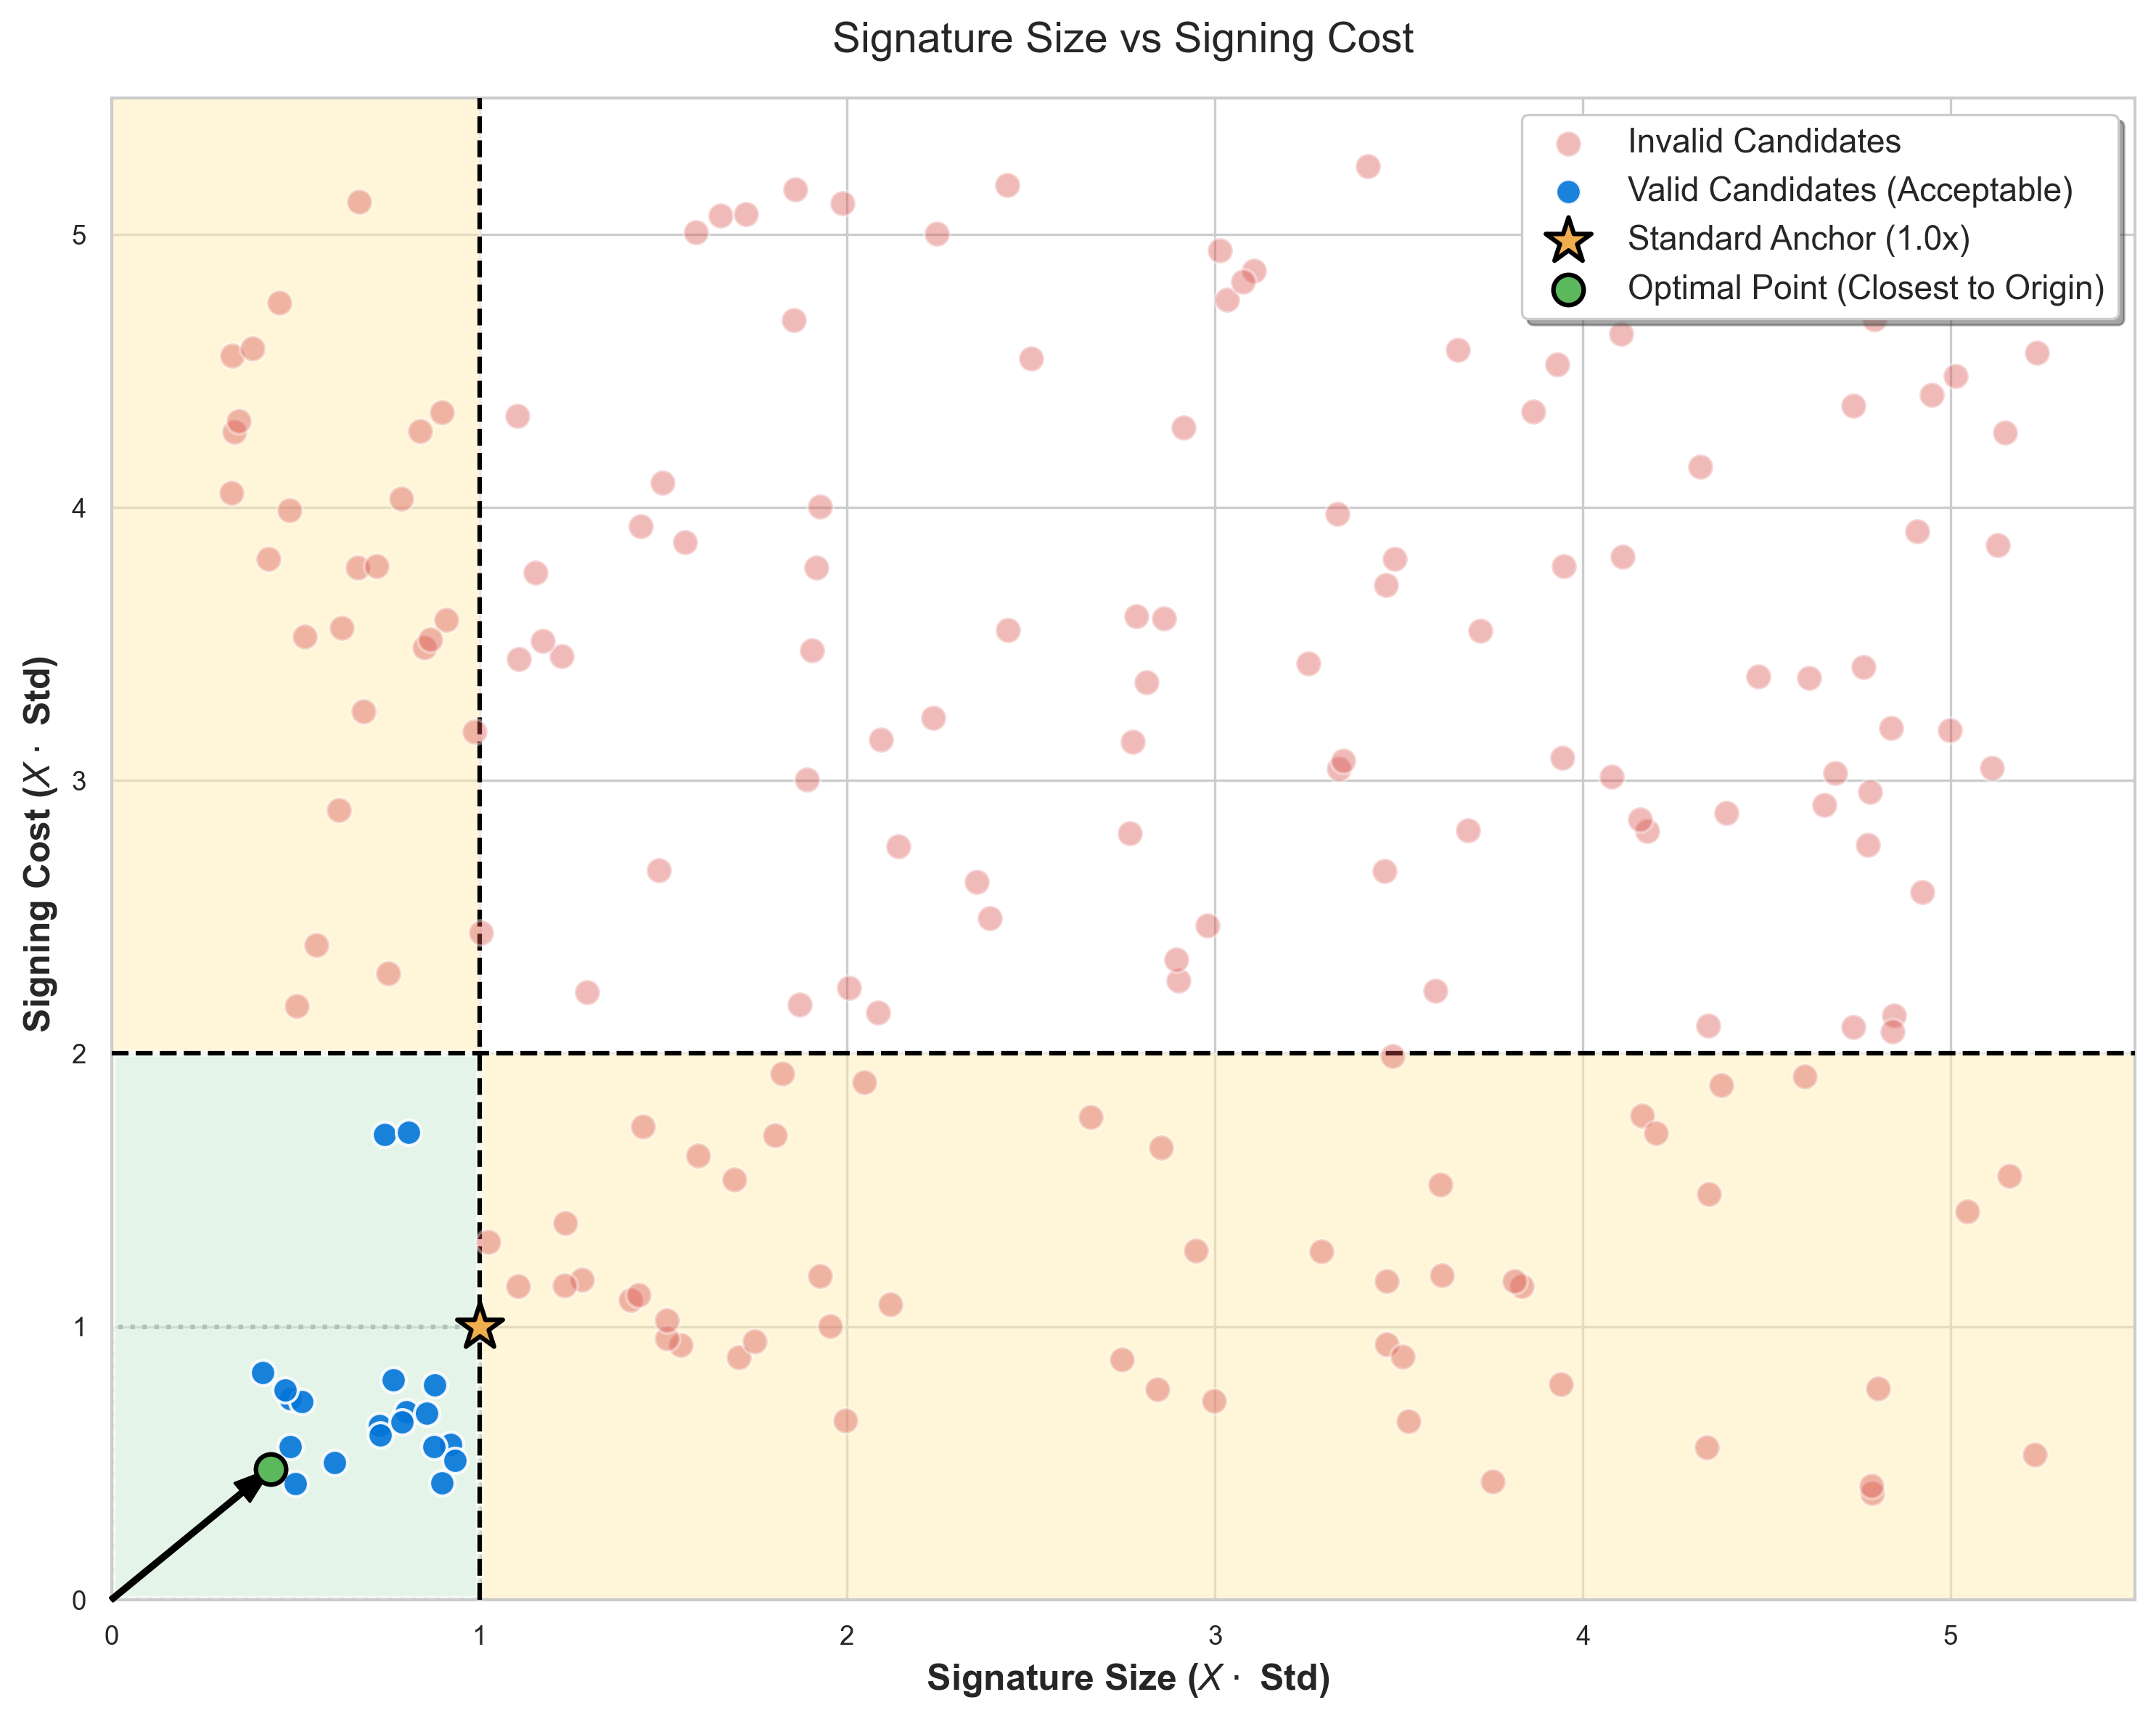
\includegraphics[width=0.7\textwidth]{content/images/scatter_plot.png}
    \caption{Visualization of Candidates with Prioritization of Size and SigGen.}
    \label{fig:scatter_plot}
\end{figure}

We cannot directly visualize a 5-dimensional space, but we can show the filtering process in a different way.

First, we scatter the unbounded candidate set (subject only to the 128-bit security condition) on a plane, with positions chosen randomly — the layout carries no meaning, and each point is uniquely identified by its parameter tuple. After initialization, we apply the signature-size filter, visualized as a colored ``sieve''. We then apply each remaining filter in turn until the last one.

The resulting set contains the candidates that survived every filter; this is the pool in which we search for the best one.

As an example, consider the following filter coefficients:
\begin{equation*}
    X_{\text{size}} = 0.85, \quad X_{\text{kg}} = 1.5, \quad X_{\text{sg}} = 2, \quad X_{\text{sv}} = 0.8, \quad X_{\text{cb}} = 1.
\end{equation*}

The filtering process is shown in Figure~\ref{fig:full_filtering_process}.

\begin{figure}[h!]
    \centering
    % Row 1
    \begin{subfigure}[b]{0.32\textwidth}
        \centering
        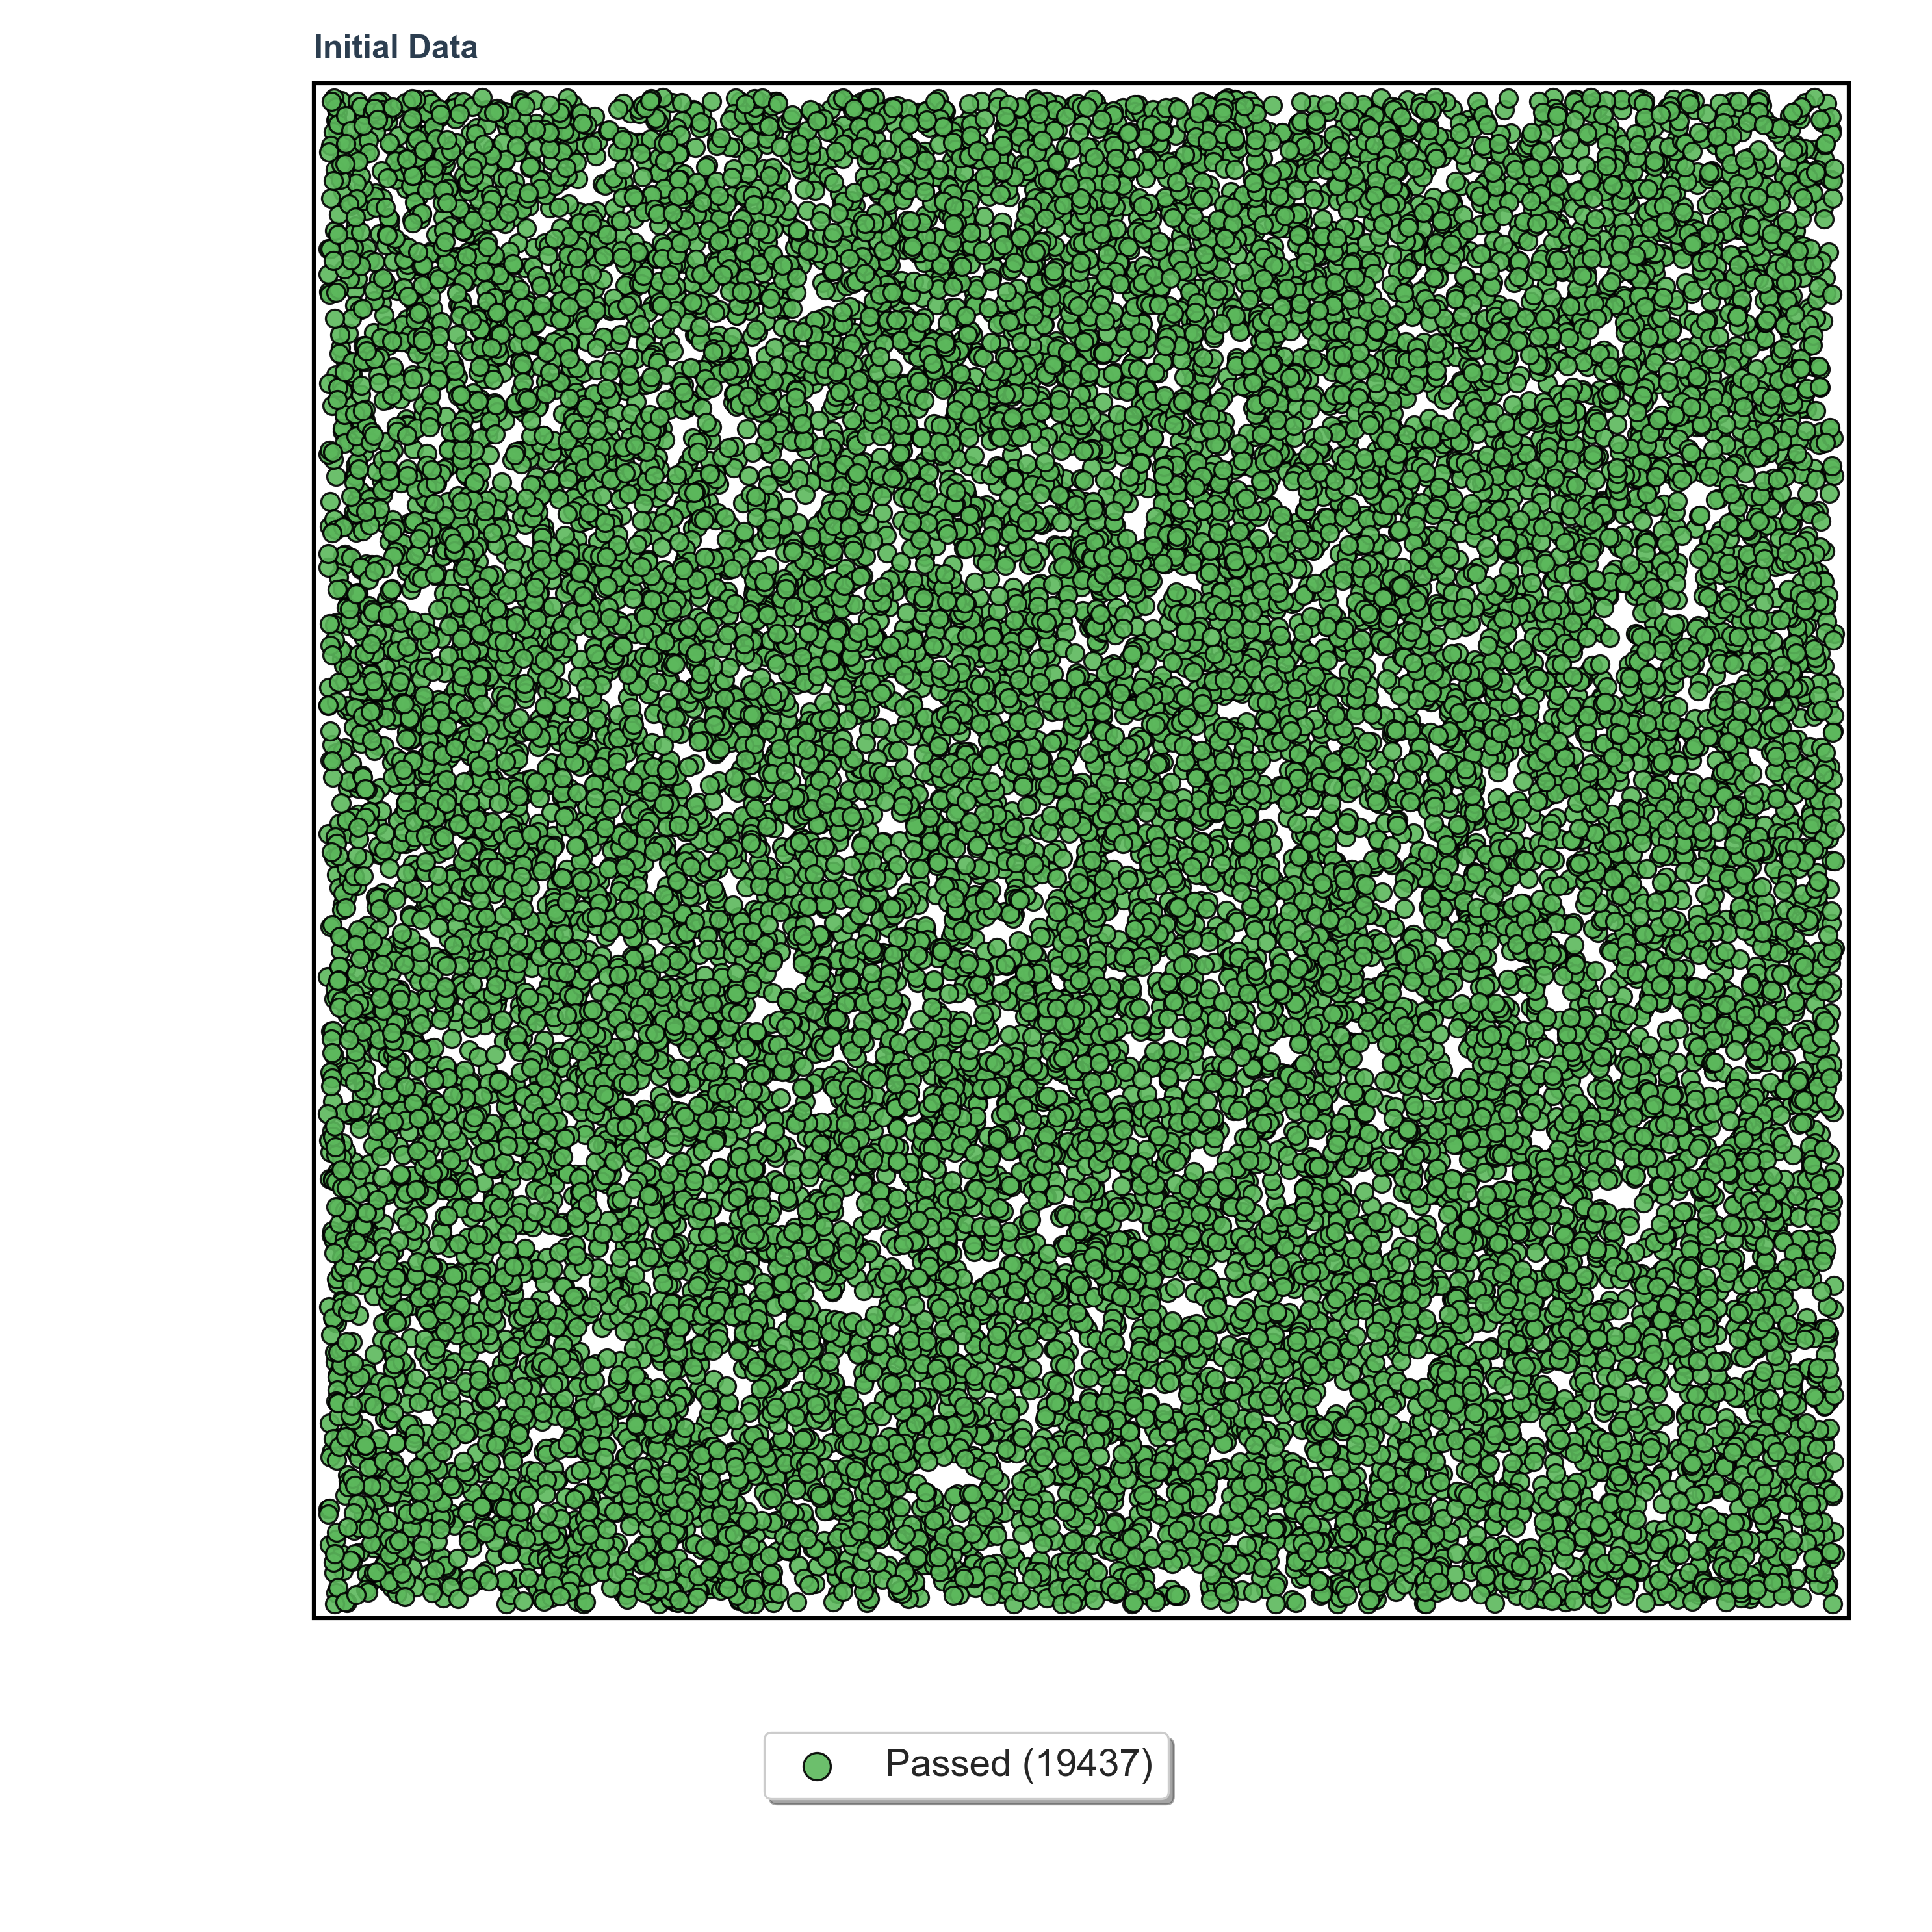
\includegraphics[width=\textwidth]{content/images/sieve_step1_initial.png}
        \caption{Initial Pool}
        \label{fig:sieve_1}
    \end{subfigure}
    \hfill
    \begin{subfigure}[b]{0.32\textwidth}
        \centering
        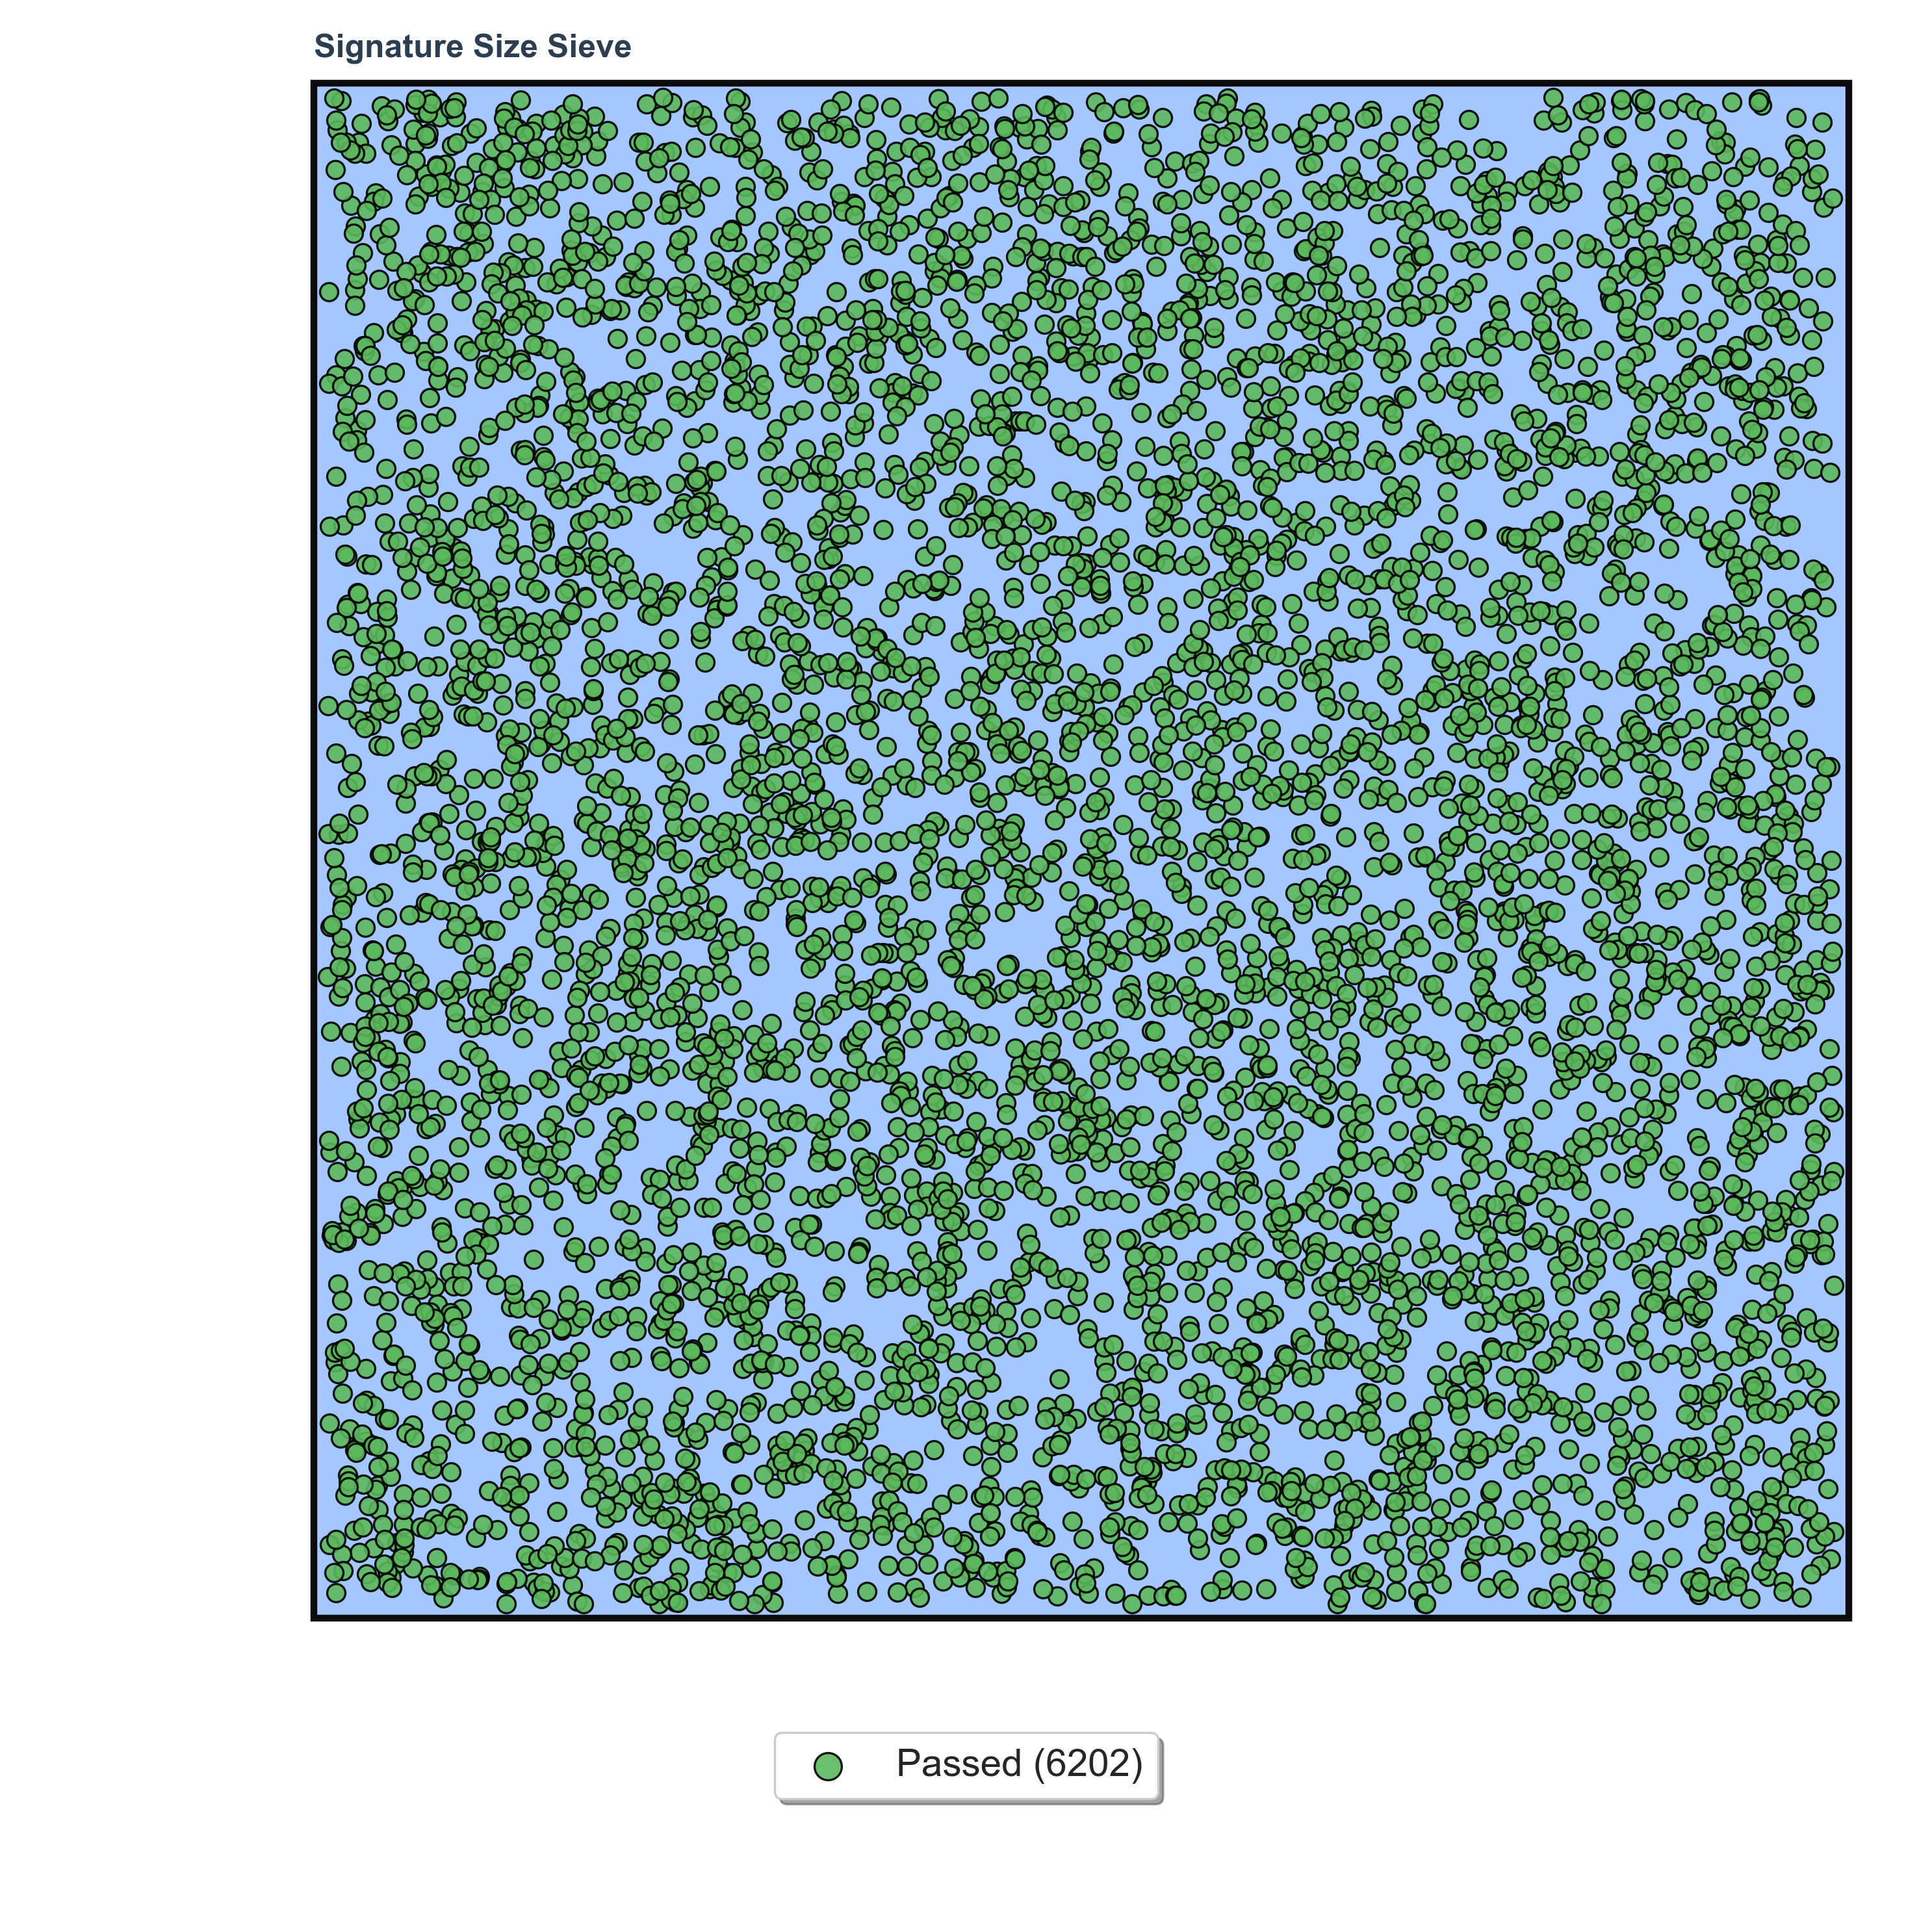
\includegraphics[width=\textwidth]{content/images/sieve_step2_size.png}
        \caption{Size}
        \label{fig:sieve_2}
    \end{subfigure}
    \hfill
    \begin{subfigure}[b]{0.32\textwidth}
        \centering
        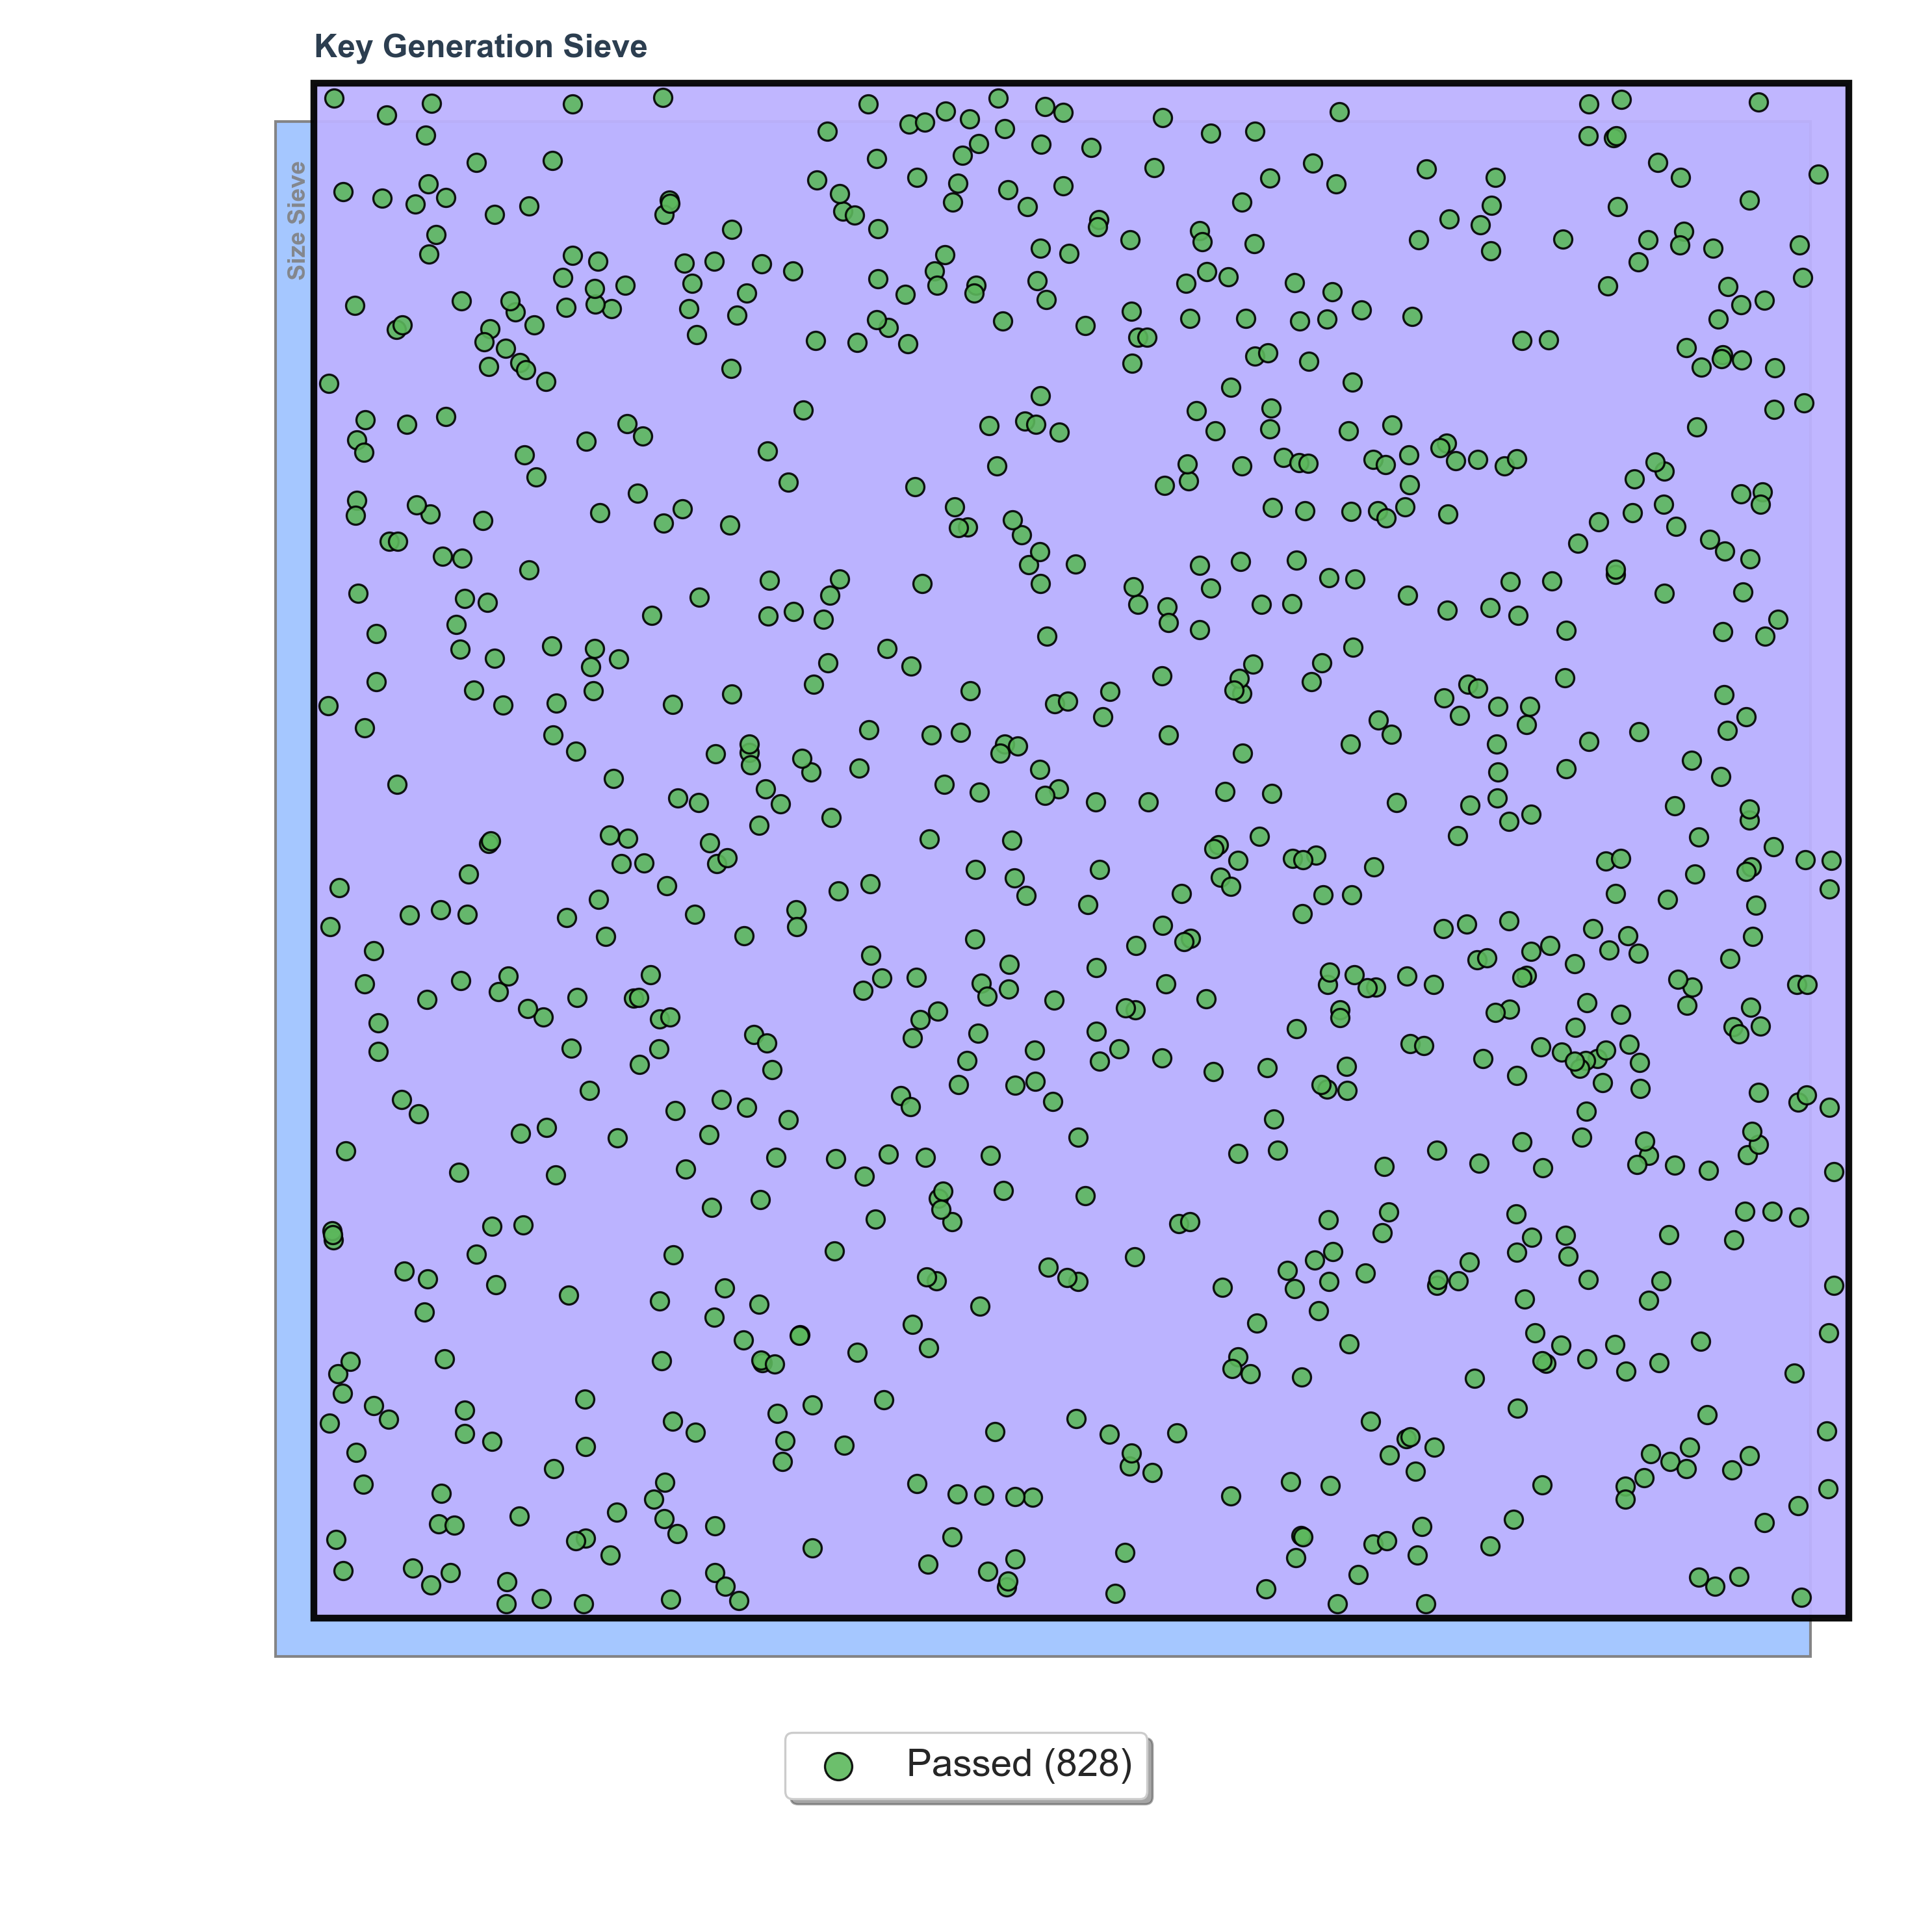
\includegraphics[width=\textwidth]{content/images/sieve_step3_keygen.png}
        \caption{KeyGen}
        \label{fig:sieve_3}
    \end{subfigure}
    
    \vspace{0.5cm}
    
    % Row 2
    \begin{subfigure}[b]{0.32\textwidth}
        \centering
        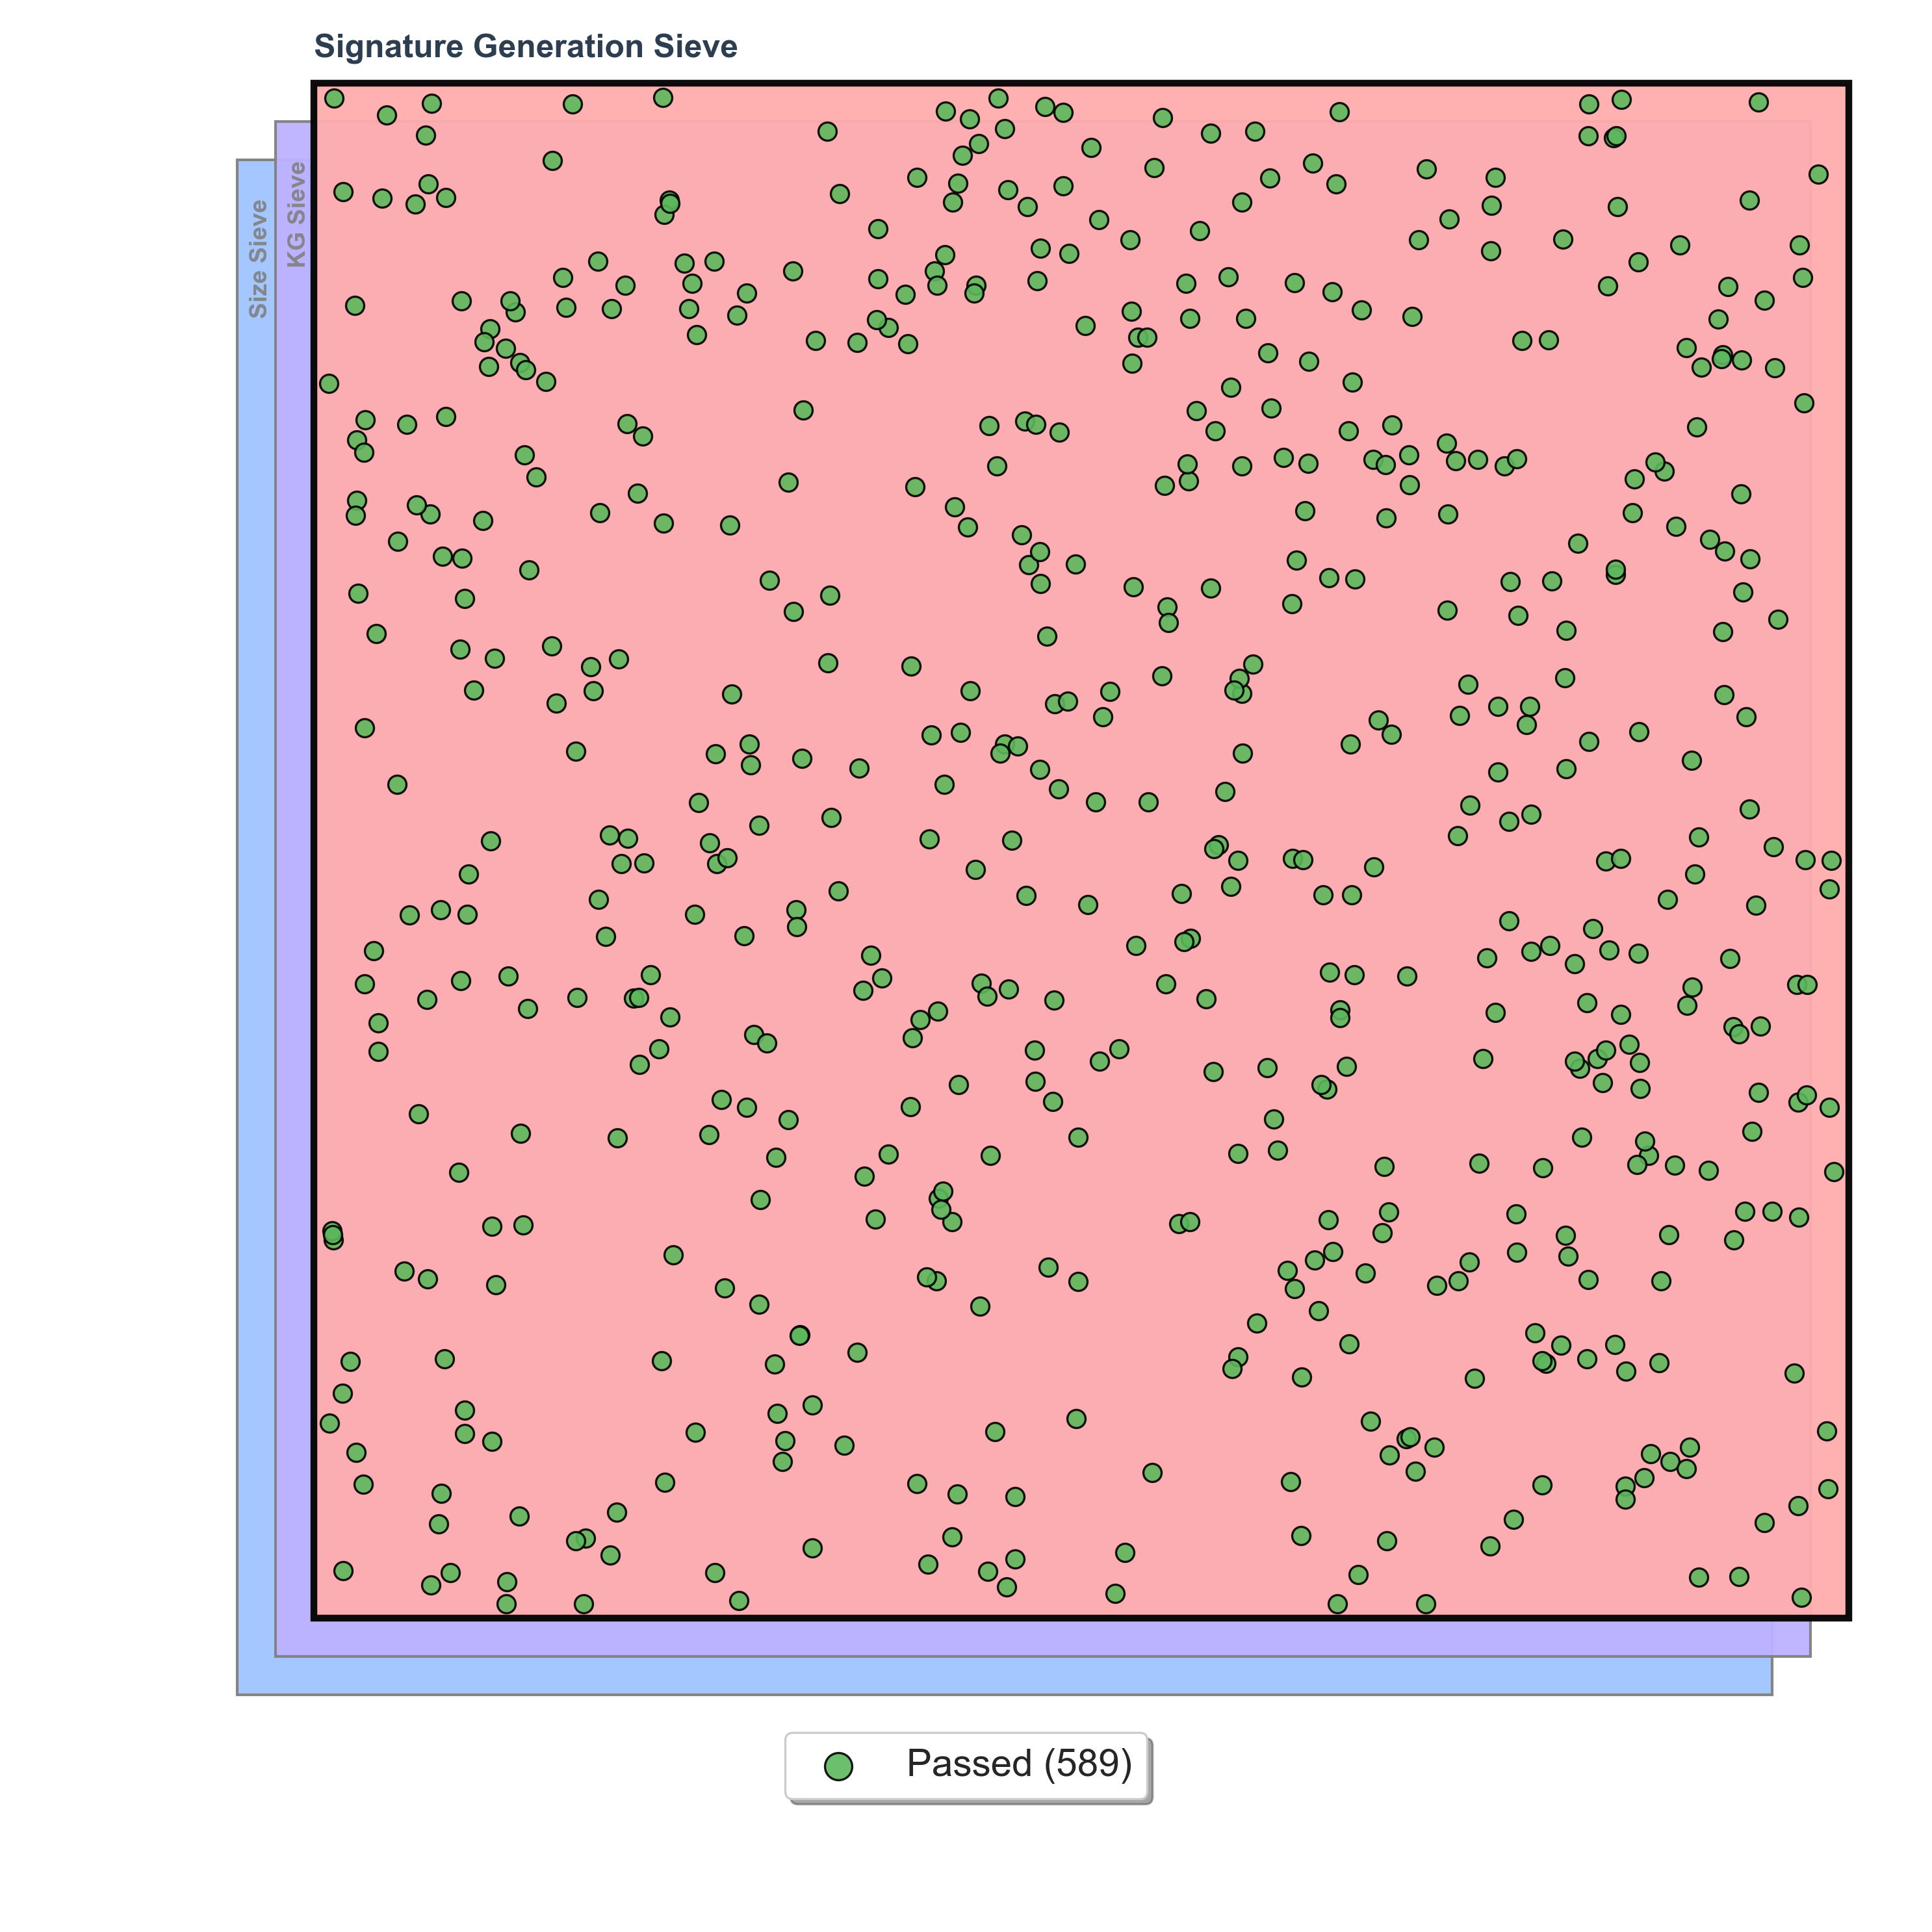
\includegraphics[width=\textwidth]{content/images/sieve_step4_siggen.png}
        \caption{SigGen}
        \label{fig:sieve_4}
    \end{subfigure}
    \hfill
    \begin{subfigure}[b]{0.32\textwidth}
        \centering
        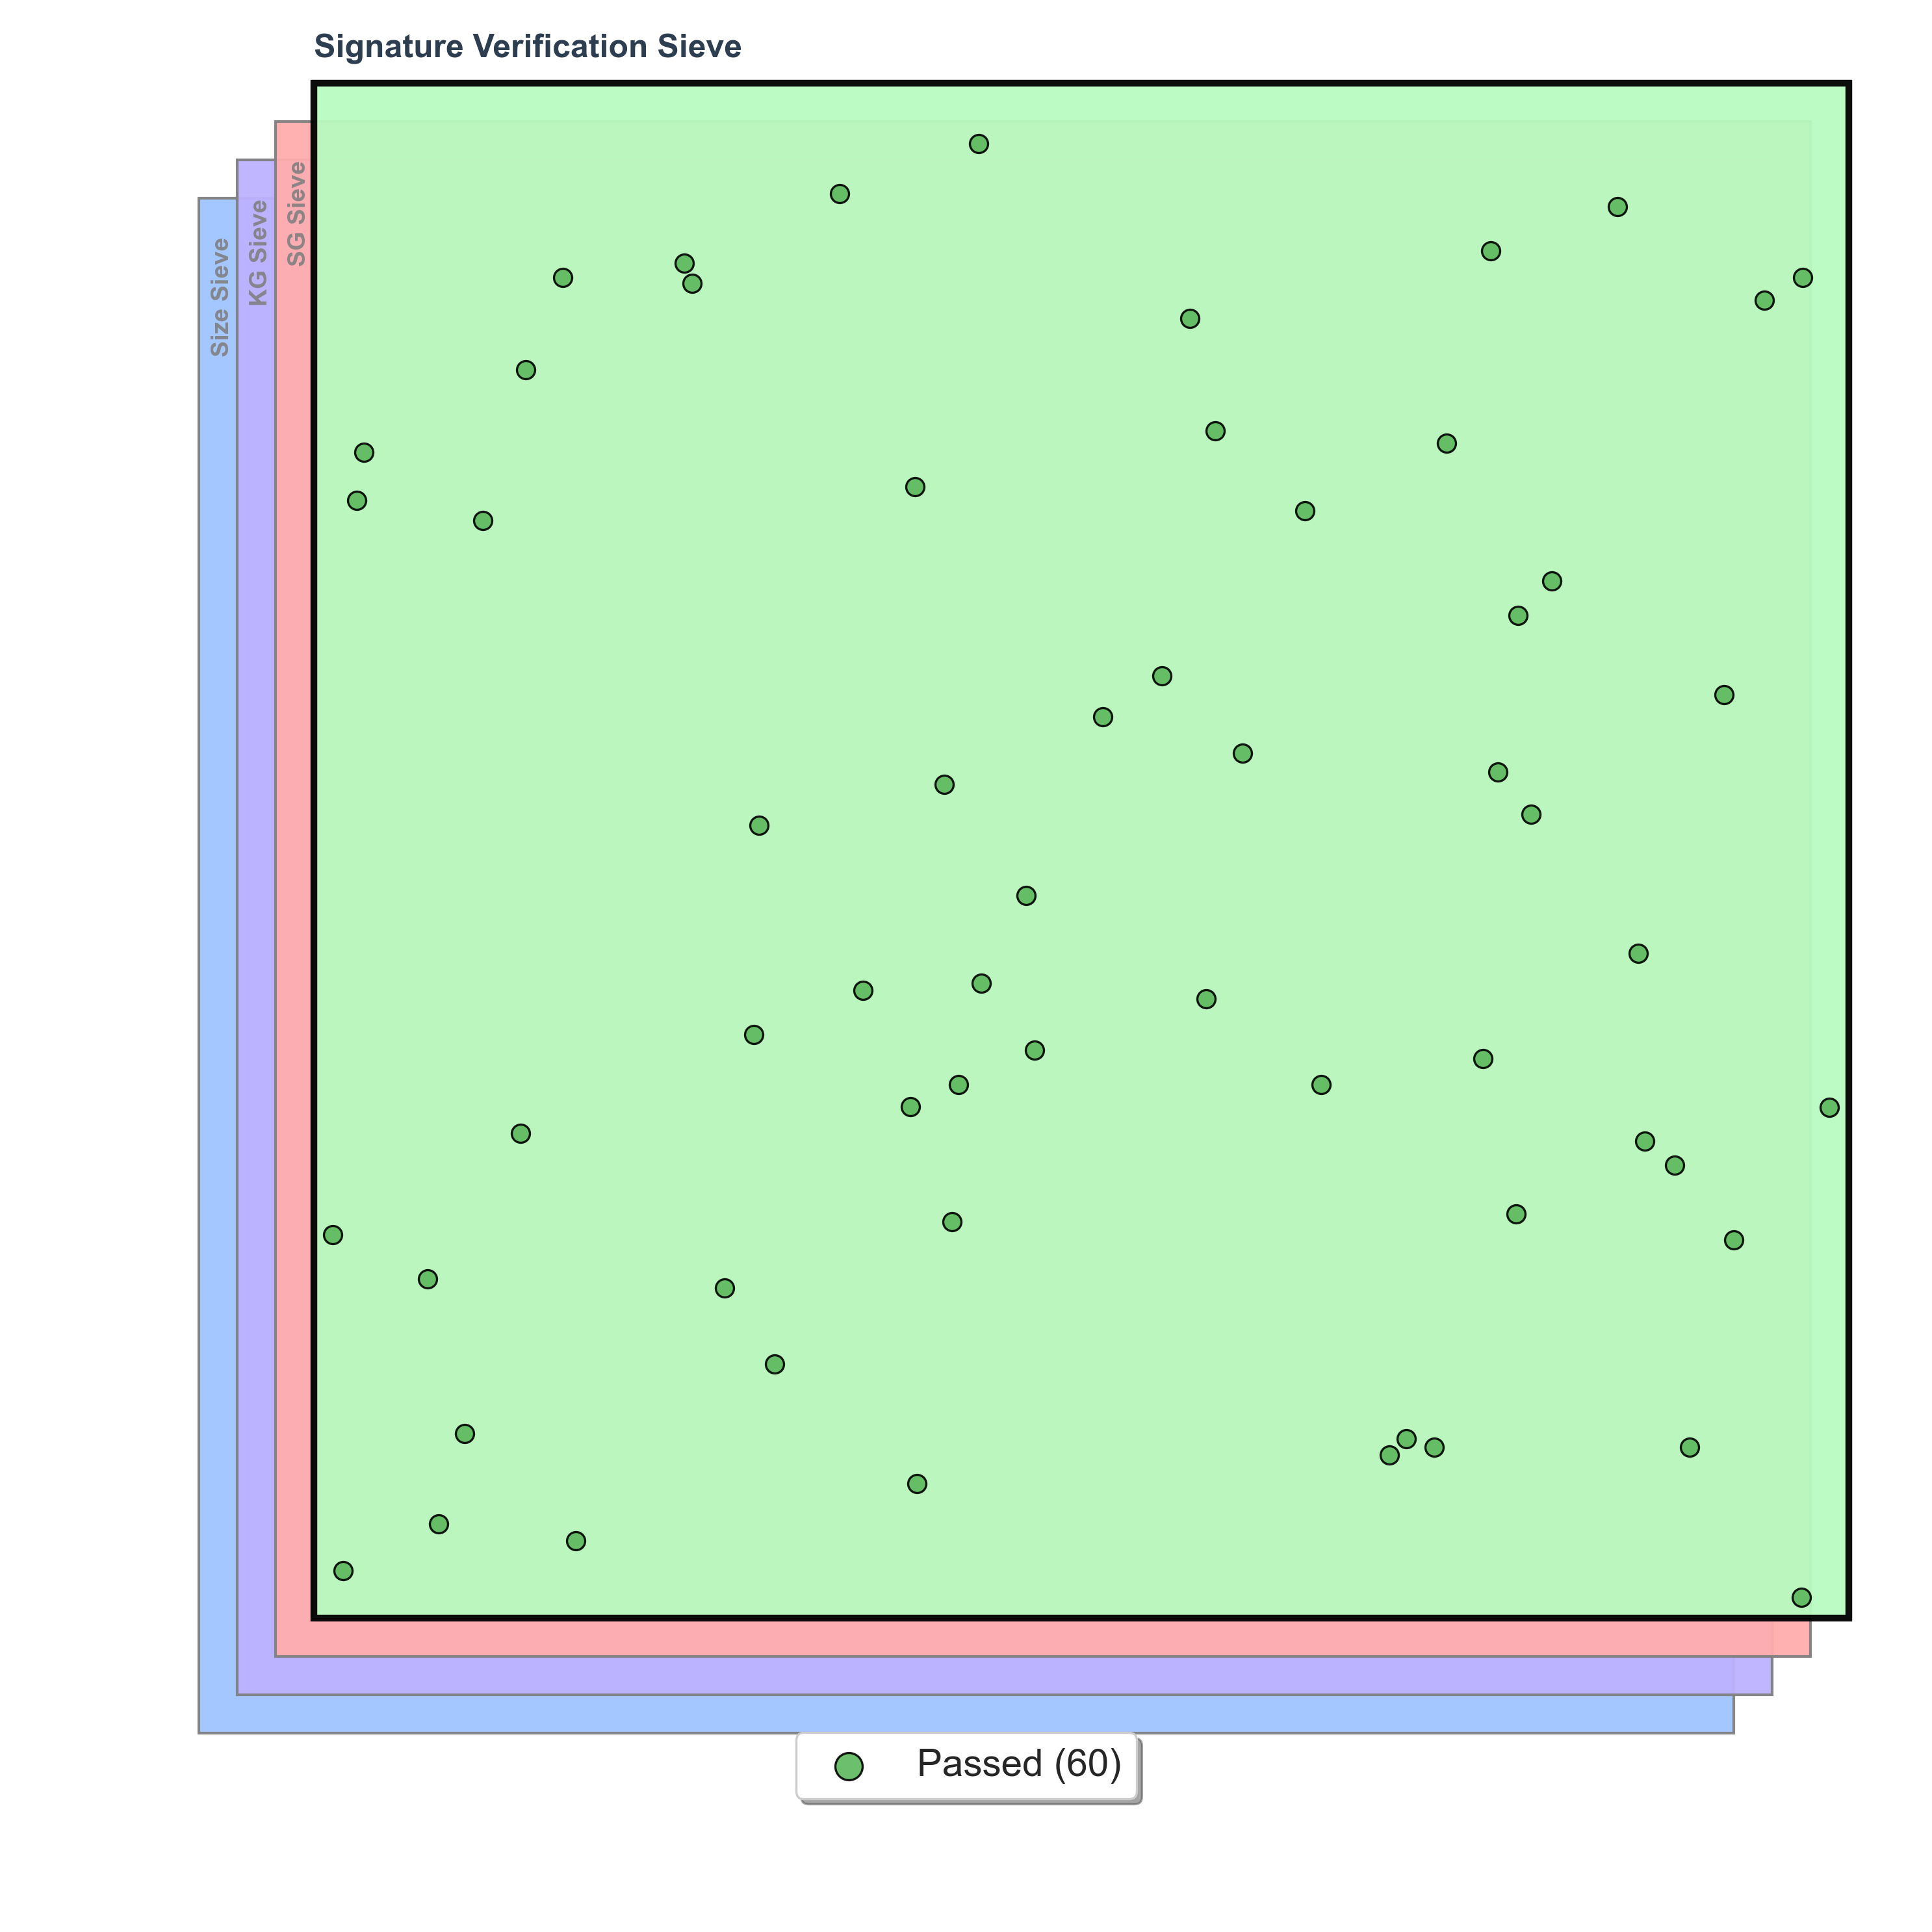
\includegraphics[width=\textwidth]{content/images/sieve_step5_verify.png}
        \caption{SigVer}
        \label{fig:sieve_5}
    \end{subfigure}
    \hfill
    \begin{subfigure}[b]{0.32\textwidth}
        \centering
        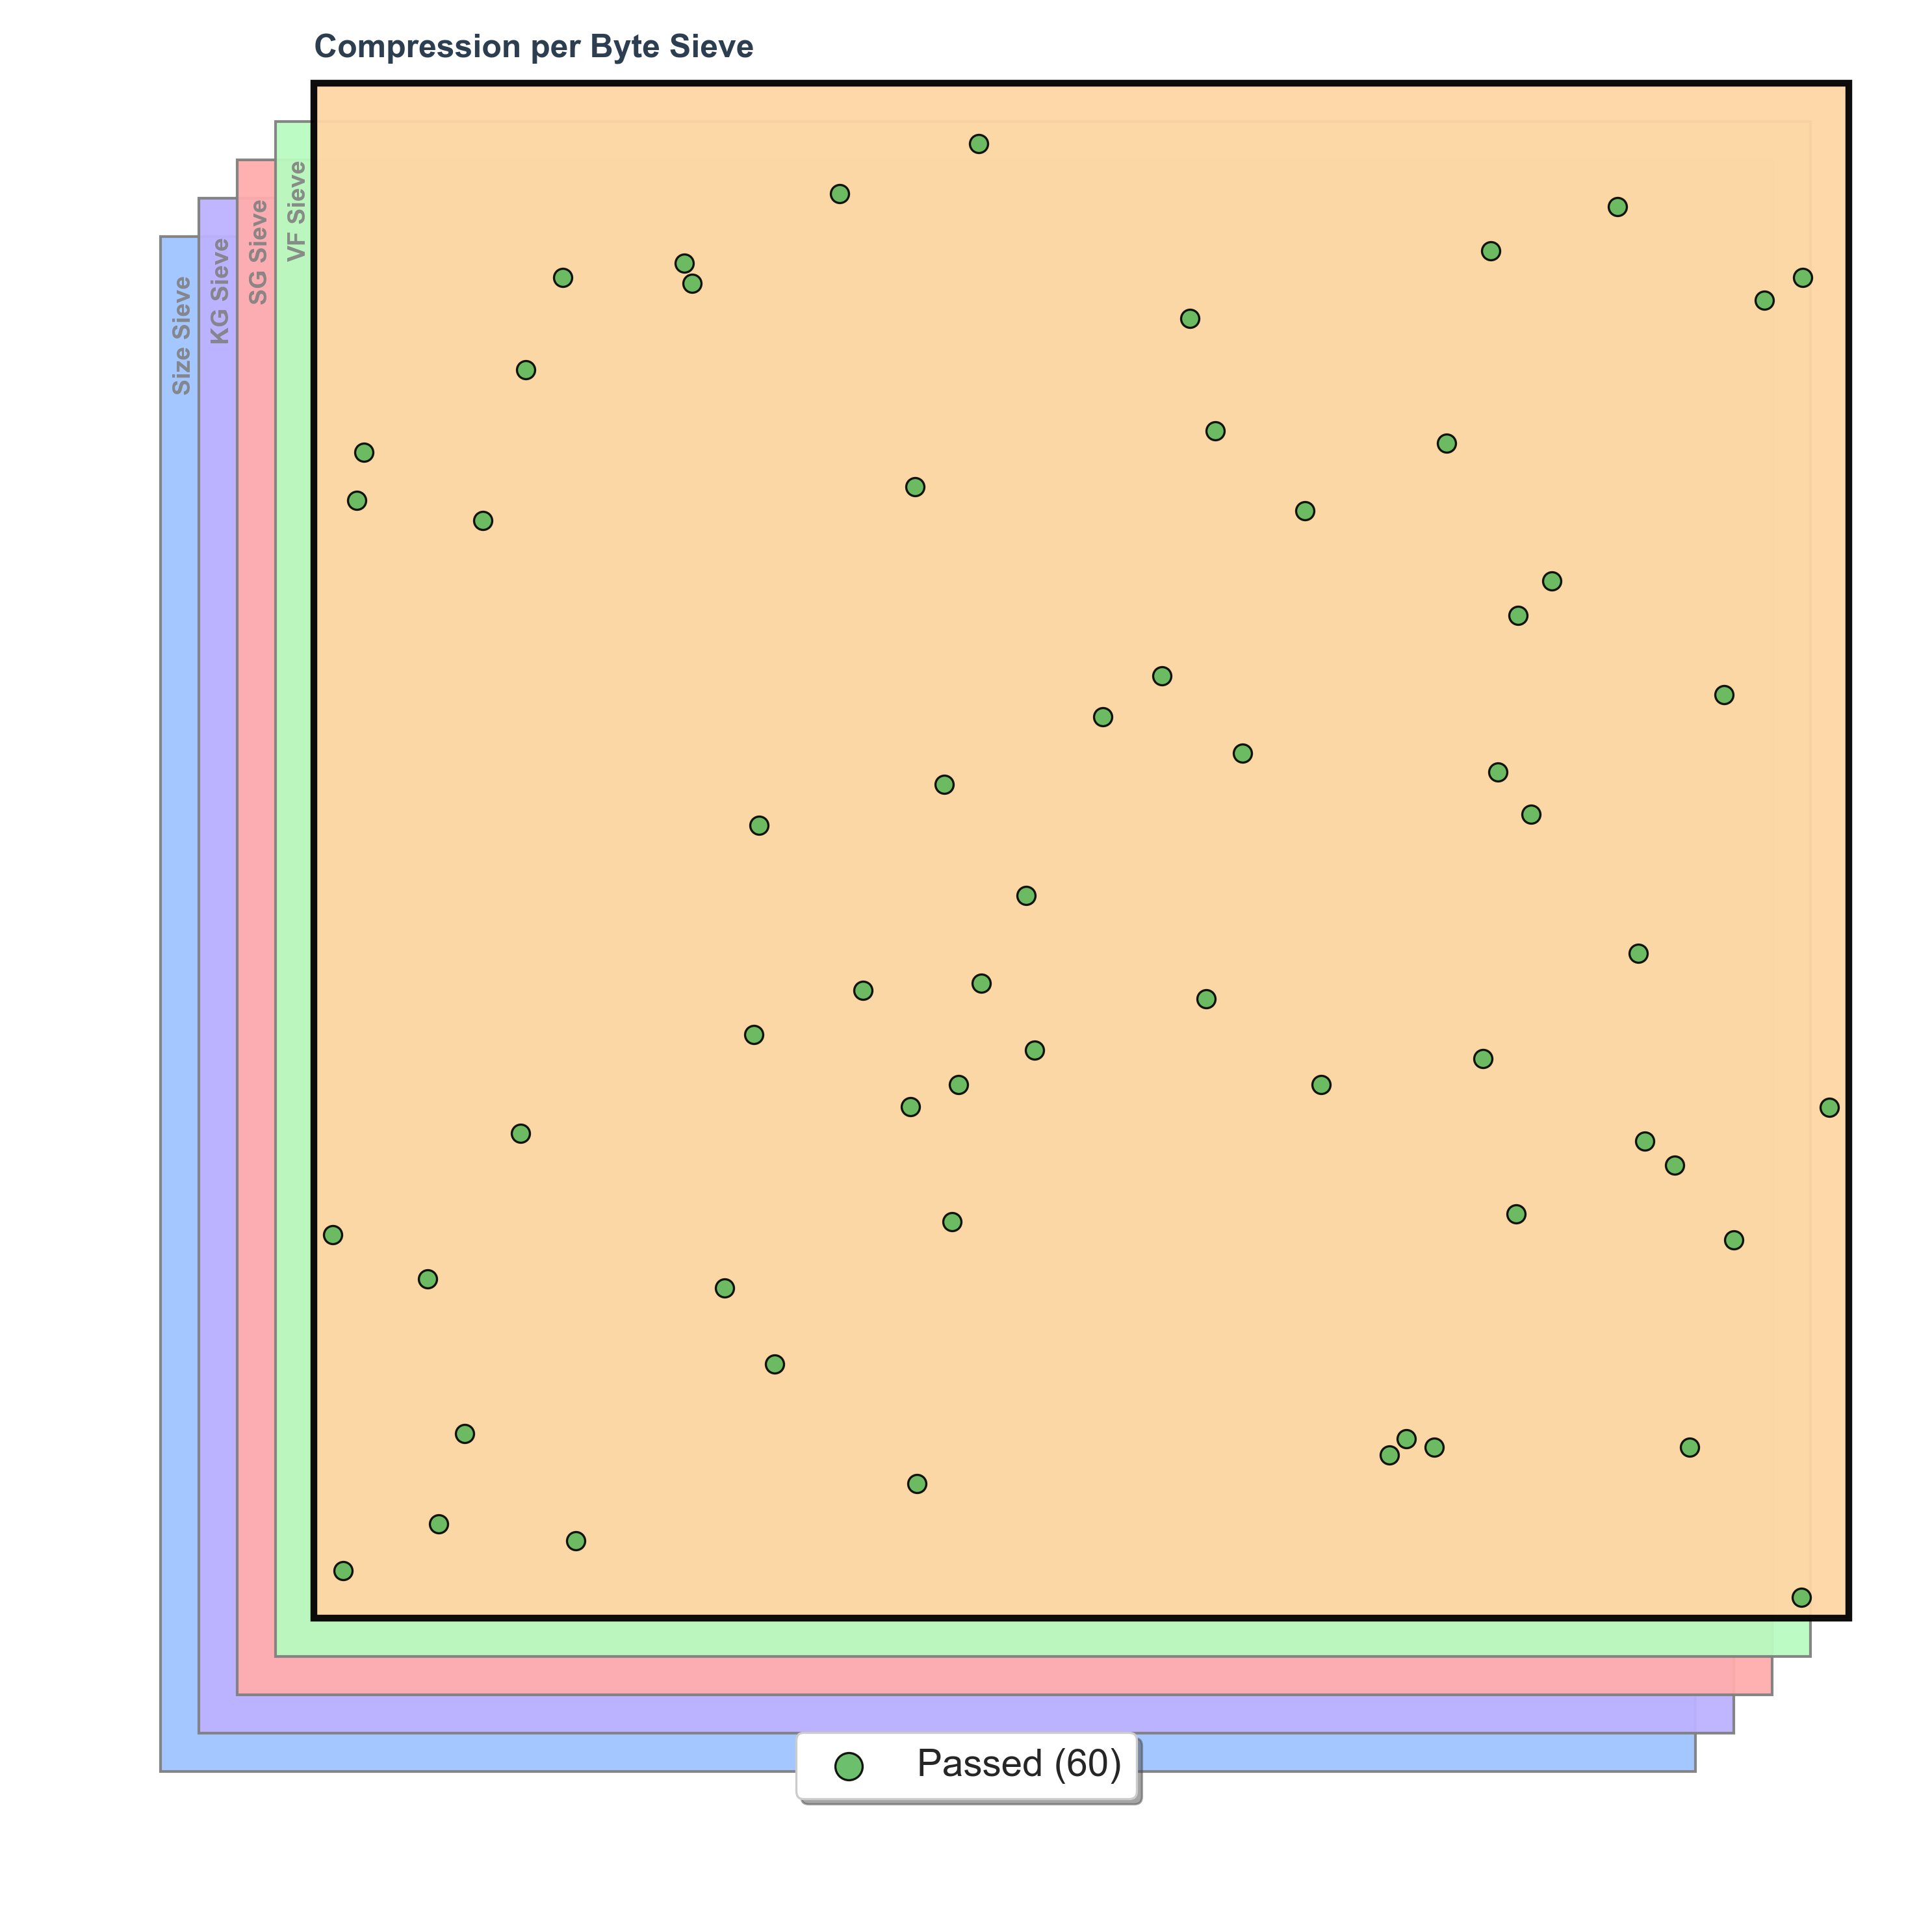
\includegraphics[width=\textwidth]{content/images/sieve_step6_rho.png}
        \caption{$\rho$}
        \label{fig:sieve_6}
    \end{subfigure}
    
    \caption{Full Parameter Filtering Process}
    \label{fig:full_filtering_process}
\end{figure}

We start with \emph{25,916} candidates. The signature-size filter trims the pool to \emph{4,814} and eliminates every $w = 2$ candidate; the next filter (KeyGen) cuts it by roughly $9\times$ and removes the last $w = 4$ candidates. Each subsequent filter prunes further, leaving \emph{61} final candidates for inspection: the verification-cost bound eliminates every $w = 256$ candidate in this example, so all survivors use $w = 16$.

With the final 61 candidates in hand, we are ready to pick a winner.

For each surviving candidate $P$, let $\widetilde{X}_i$ denote the ratio of the candidate's value for metric $i$ to the corresponding standard value, where $i \in \{\text{size}, \text{kg}, \text{sg}, \text{sv}, \text{cb}\}$. Working with ratios rather than raw values keeps the five axes on a common, dimensionless scale. The Euclidean distance from the origin to $P$ is then
\begin{equation}
    d(P) = \sqrt{\widetilde{X}_{\text{size}}^2 + \widetilde{X}_{\text{kg}}^2 + \widetilde{X}_{\text{sg}}^2 + \widetilde{X}_{\text{sv}}^2 + \widetilde{X}_{\text{cb}}^2}\,,
    \label{eq:euclidean_distance}
\end{equation}
and the optimal candidate is the one minimizing $d(P)$.

This treats every metric as equally important, which is rarely what we actually want. Signature size, for example, usually carries far more weight than key-generation cost in a Bitcoin context. The next subsection addresses this by attaching weights to each axis.

\subsection{Decisional Weights} \label{sec:decisional-weights}
We can do better by applying the \emph{weighted} Euclidean distance. The motivation is that weights give us a principled way to encode the relative priority of each metric. Let $w_{\text{size}}, w_{\text{kg}}, w_{\text{sg}}, w_{\text{sv}}, w_{\text{cb}} \in \mathbb{R}^+$ denote the raw weight coefficients representing the relative importance of size, KeyGen, SigGen, SigVer and $\rho$, respectively.

To keep the calculation proportionally consistent regardless of the absolute scale of the chosen weights, we normalize them into coefficients $p_i$ (where $i \in \{\text{size}, \text{kg}, \text{sg}, \text{sv}, \text{cb}\}$) such that they sum to $1$:
\begin{equation}
    p_i = \frac{w_i}{w_{\text{size}} + w_{\text{kg}} + w_{\text{sg}} + w_{\text{sv}} + w_{\text{cb}}}, \quad \text{ensuring} \quad \sum p_i = 1
    \label{eq:weight_normalization}
\end{equation}

Using these normalized coefficients, we calculate the Weighted Euclidean Distance (the $L_2$ norm) from the origin $(0,0,0,0,0)$ to the candidate's point $P$. The distance $d(P)$ is defined as:
\begin{equation}
    d(P) = \sqrt{p_{\text{size}} \widetilde{X}_{\text{size}}^2 + p_{\text{kg}} \widetilde{X}_{\text{kg}}^2 + p_{\text{sg}} \widetilde{X}_{\text{sg}}^2 + p_{\text{sv}} \widetilde{X}_{\text{sv}}^2 + p_{\text{cb}} \widetilde{X}_{\text{cb}}^2}
    \label{eq:weighted_euclidean_distance}
\end{equation}

As before, each $\widetilde{X}_i$ is the ratio of the candidate's metric to its standard counterpart, so the five axes remain on a common dimensionless scale.

To visualize the distances, we map each candidate's distance onto a color scale: lower distances shade towards blue, higher distances towards red. As an example, consider the following two weight settings:
\begin{itemize}
    \item Case 1: $w_{\text{size}} = w_{\text{kg}} = w_{\text{sg}} = w_{\text{sv}} = w_{\text{cb}} = 1$;
    \item Case 2: $w_{\text{size}} = 5,\ w_{\text{kg}} = 1,\ w_{\text{sg}} = 1.5,\ w_{\text{sv}} = 2,\ w_{\text{cb}} = 1$.
\end{itemize}

The result for the first case is shown below.

\begin{figure}[htbp]
    \centering
    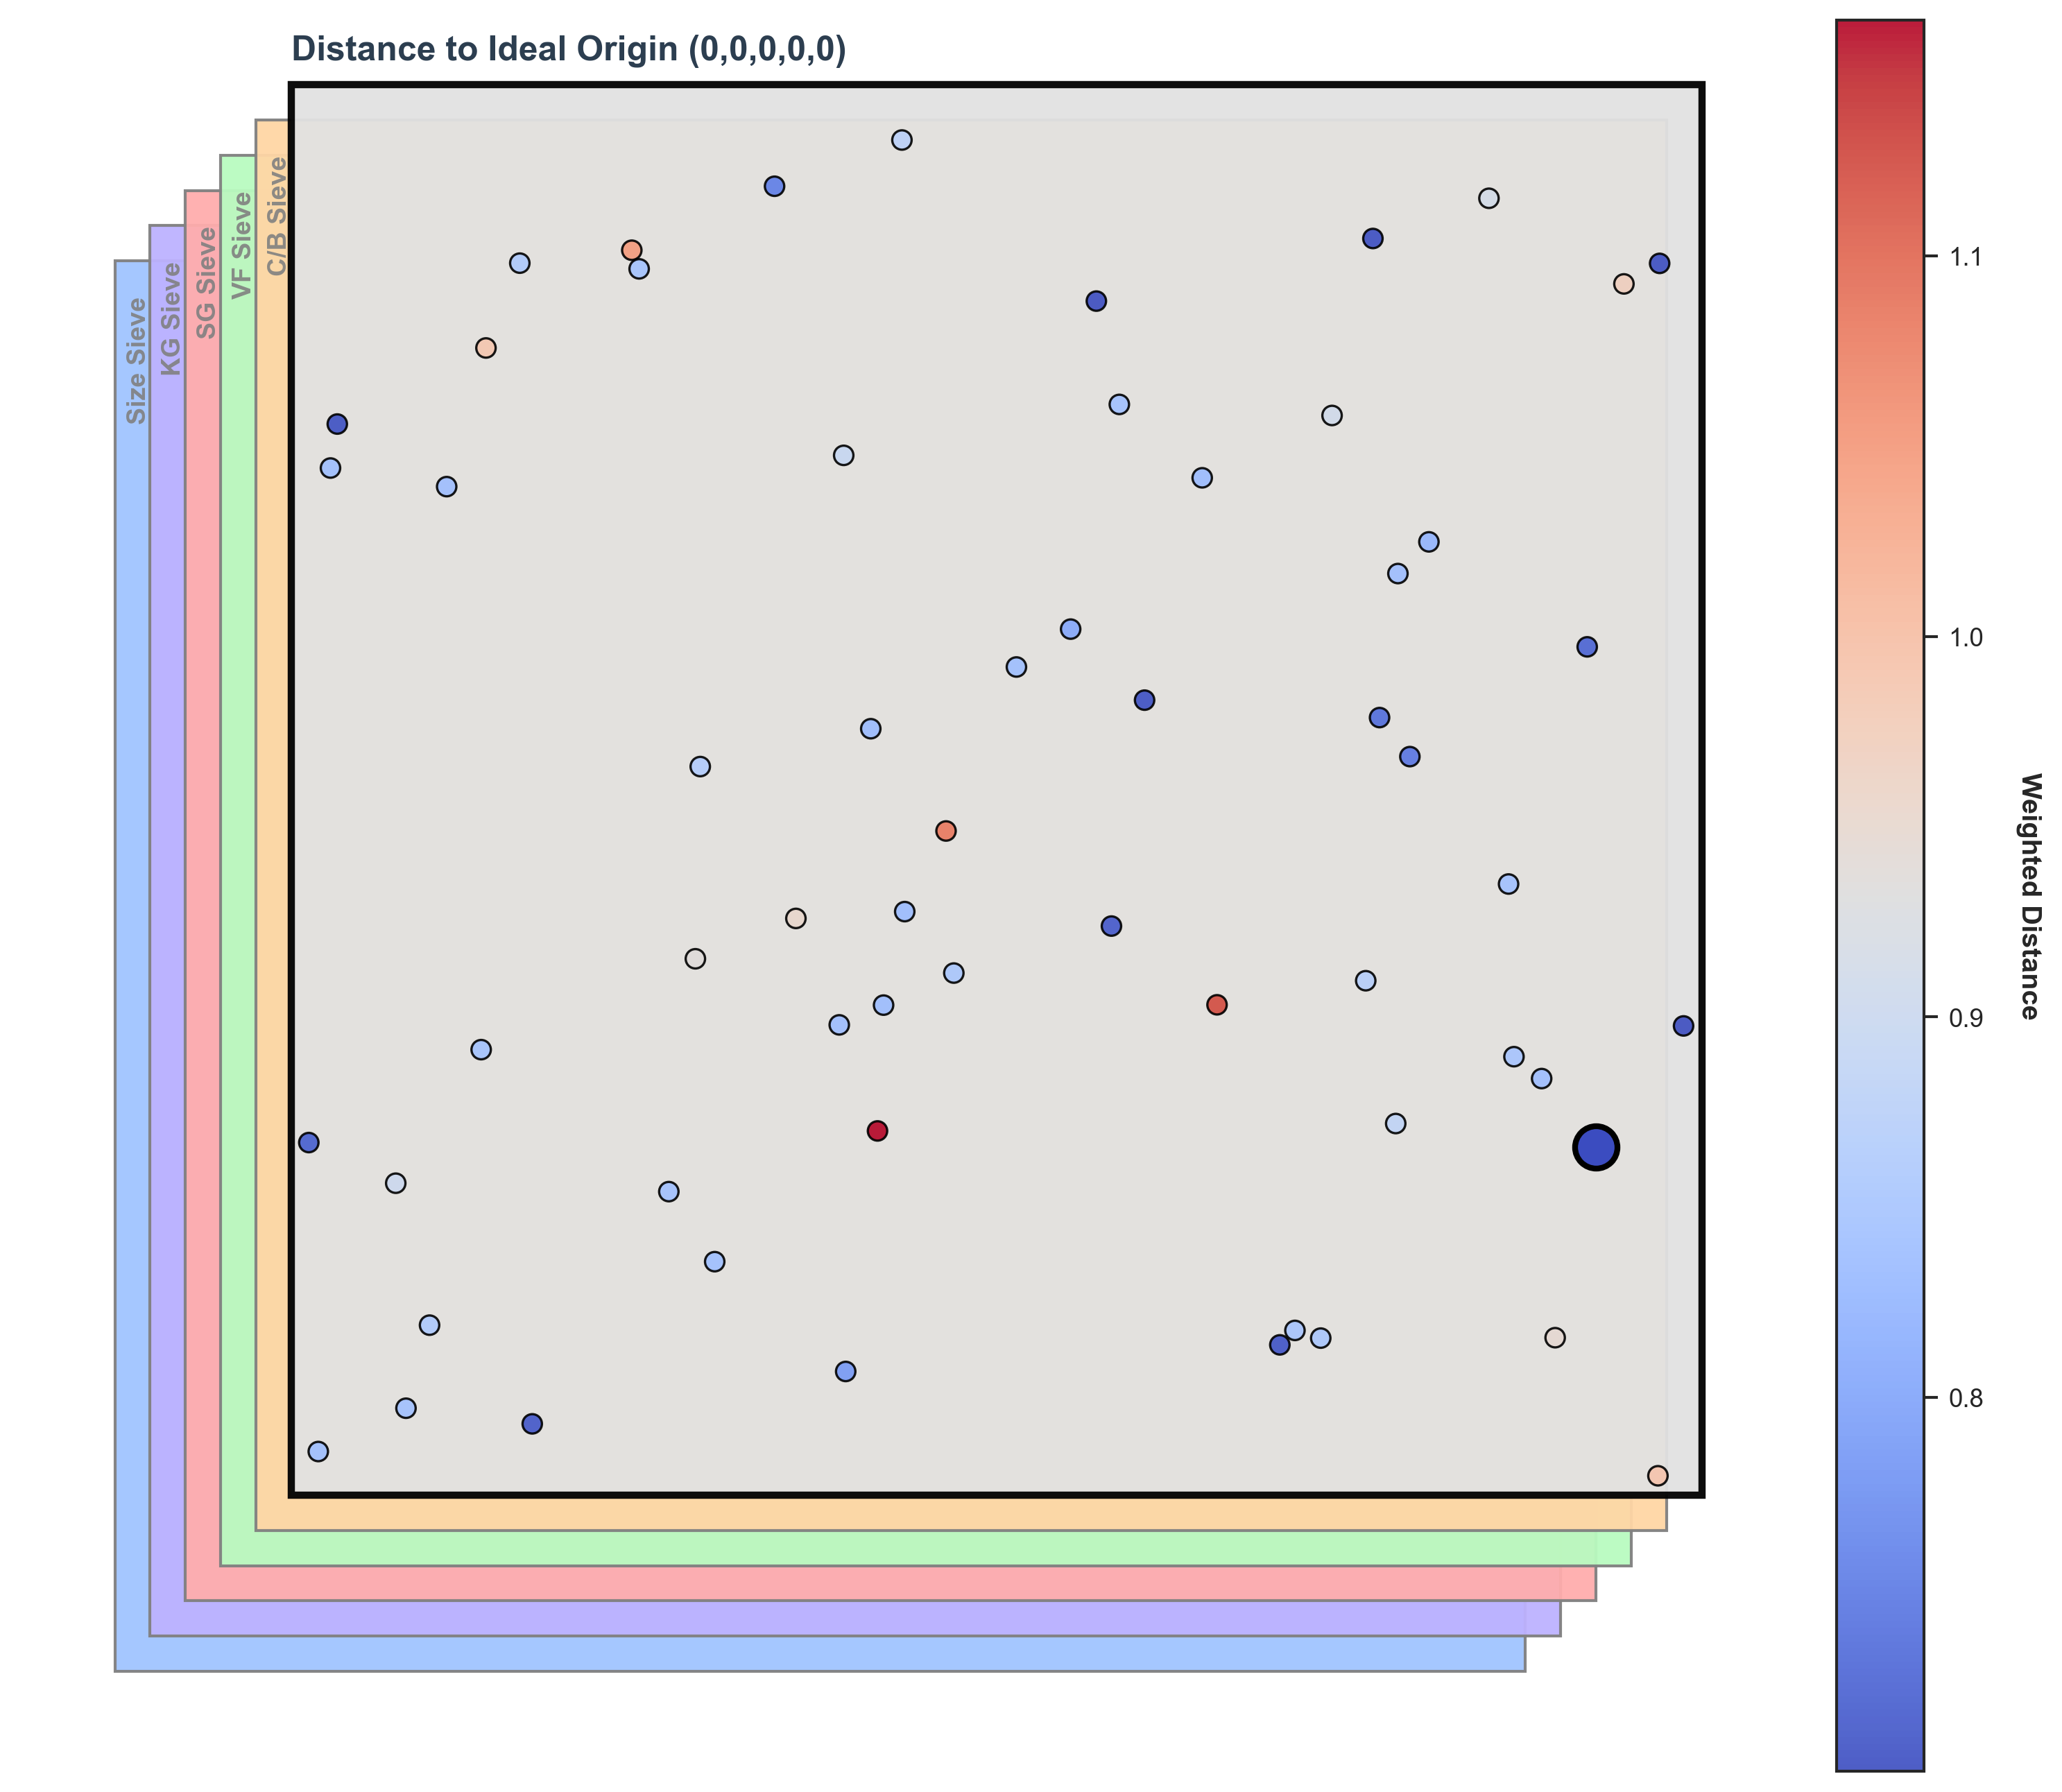
\includegraphics[width=0.75\textwidth]{content/images/sieve_step7_distance_1.png}
    \caption{Visualization of the Search for Case 1.}
    \label{fig:distance_plot_1}
\end{figure}

The parameters and metric values of the best candidate are shown in Table~\ref{tab:euclidean_candidate_metrics_case_1}.


\begin{table}[htbp]
    \centering
    \small
    \caption{Performance Comparison between the Standard Baseline and the Best Shortest Distance Candidate}
    \label{tab:euclidean_candidate_metrics_case_1}
    \begin{tabular}{lrrr}
        \toprule
        \textbf{Metric} & \textbf{Standard Baseline} & \textbf{Best Candidate} & \textbf{Ratio to Std.} \\
        \midrule
        Parameters $(h, d, k, a, w)$ & $(63, 7, 14, 12, 16)$ & $(40, 5, 19, 9, 16)$ & -- \\
        Size (B) & $7,856$ & $6,496$ & $0.8269\times$ \\
        KeyGen ($C$) & $292,351$ & $146,175$ & $0.5000\times$ \\
        SigGen ($C$) & $2,218,486$ & $760,053$ & $0.3426\times$ \\
        SigVer ($C$) & $2,193$ & $1,626$ & $0.7415\times$ \\
        $\rho$ ($C$/B) & $0.2791$ & $0.2503$ & $0.8967\times$ \\
        \bottomrule
    \end{tabular}
\end{table}

\newpage

For the second case, we have the following picture:

\begin{figure}[htbp]
    \centering
    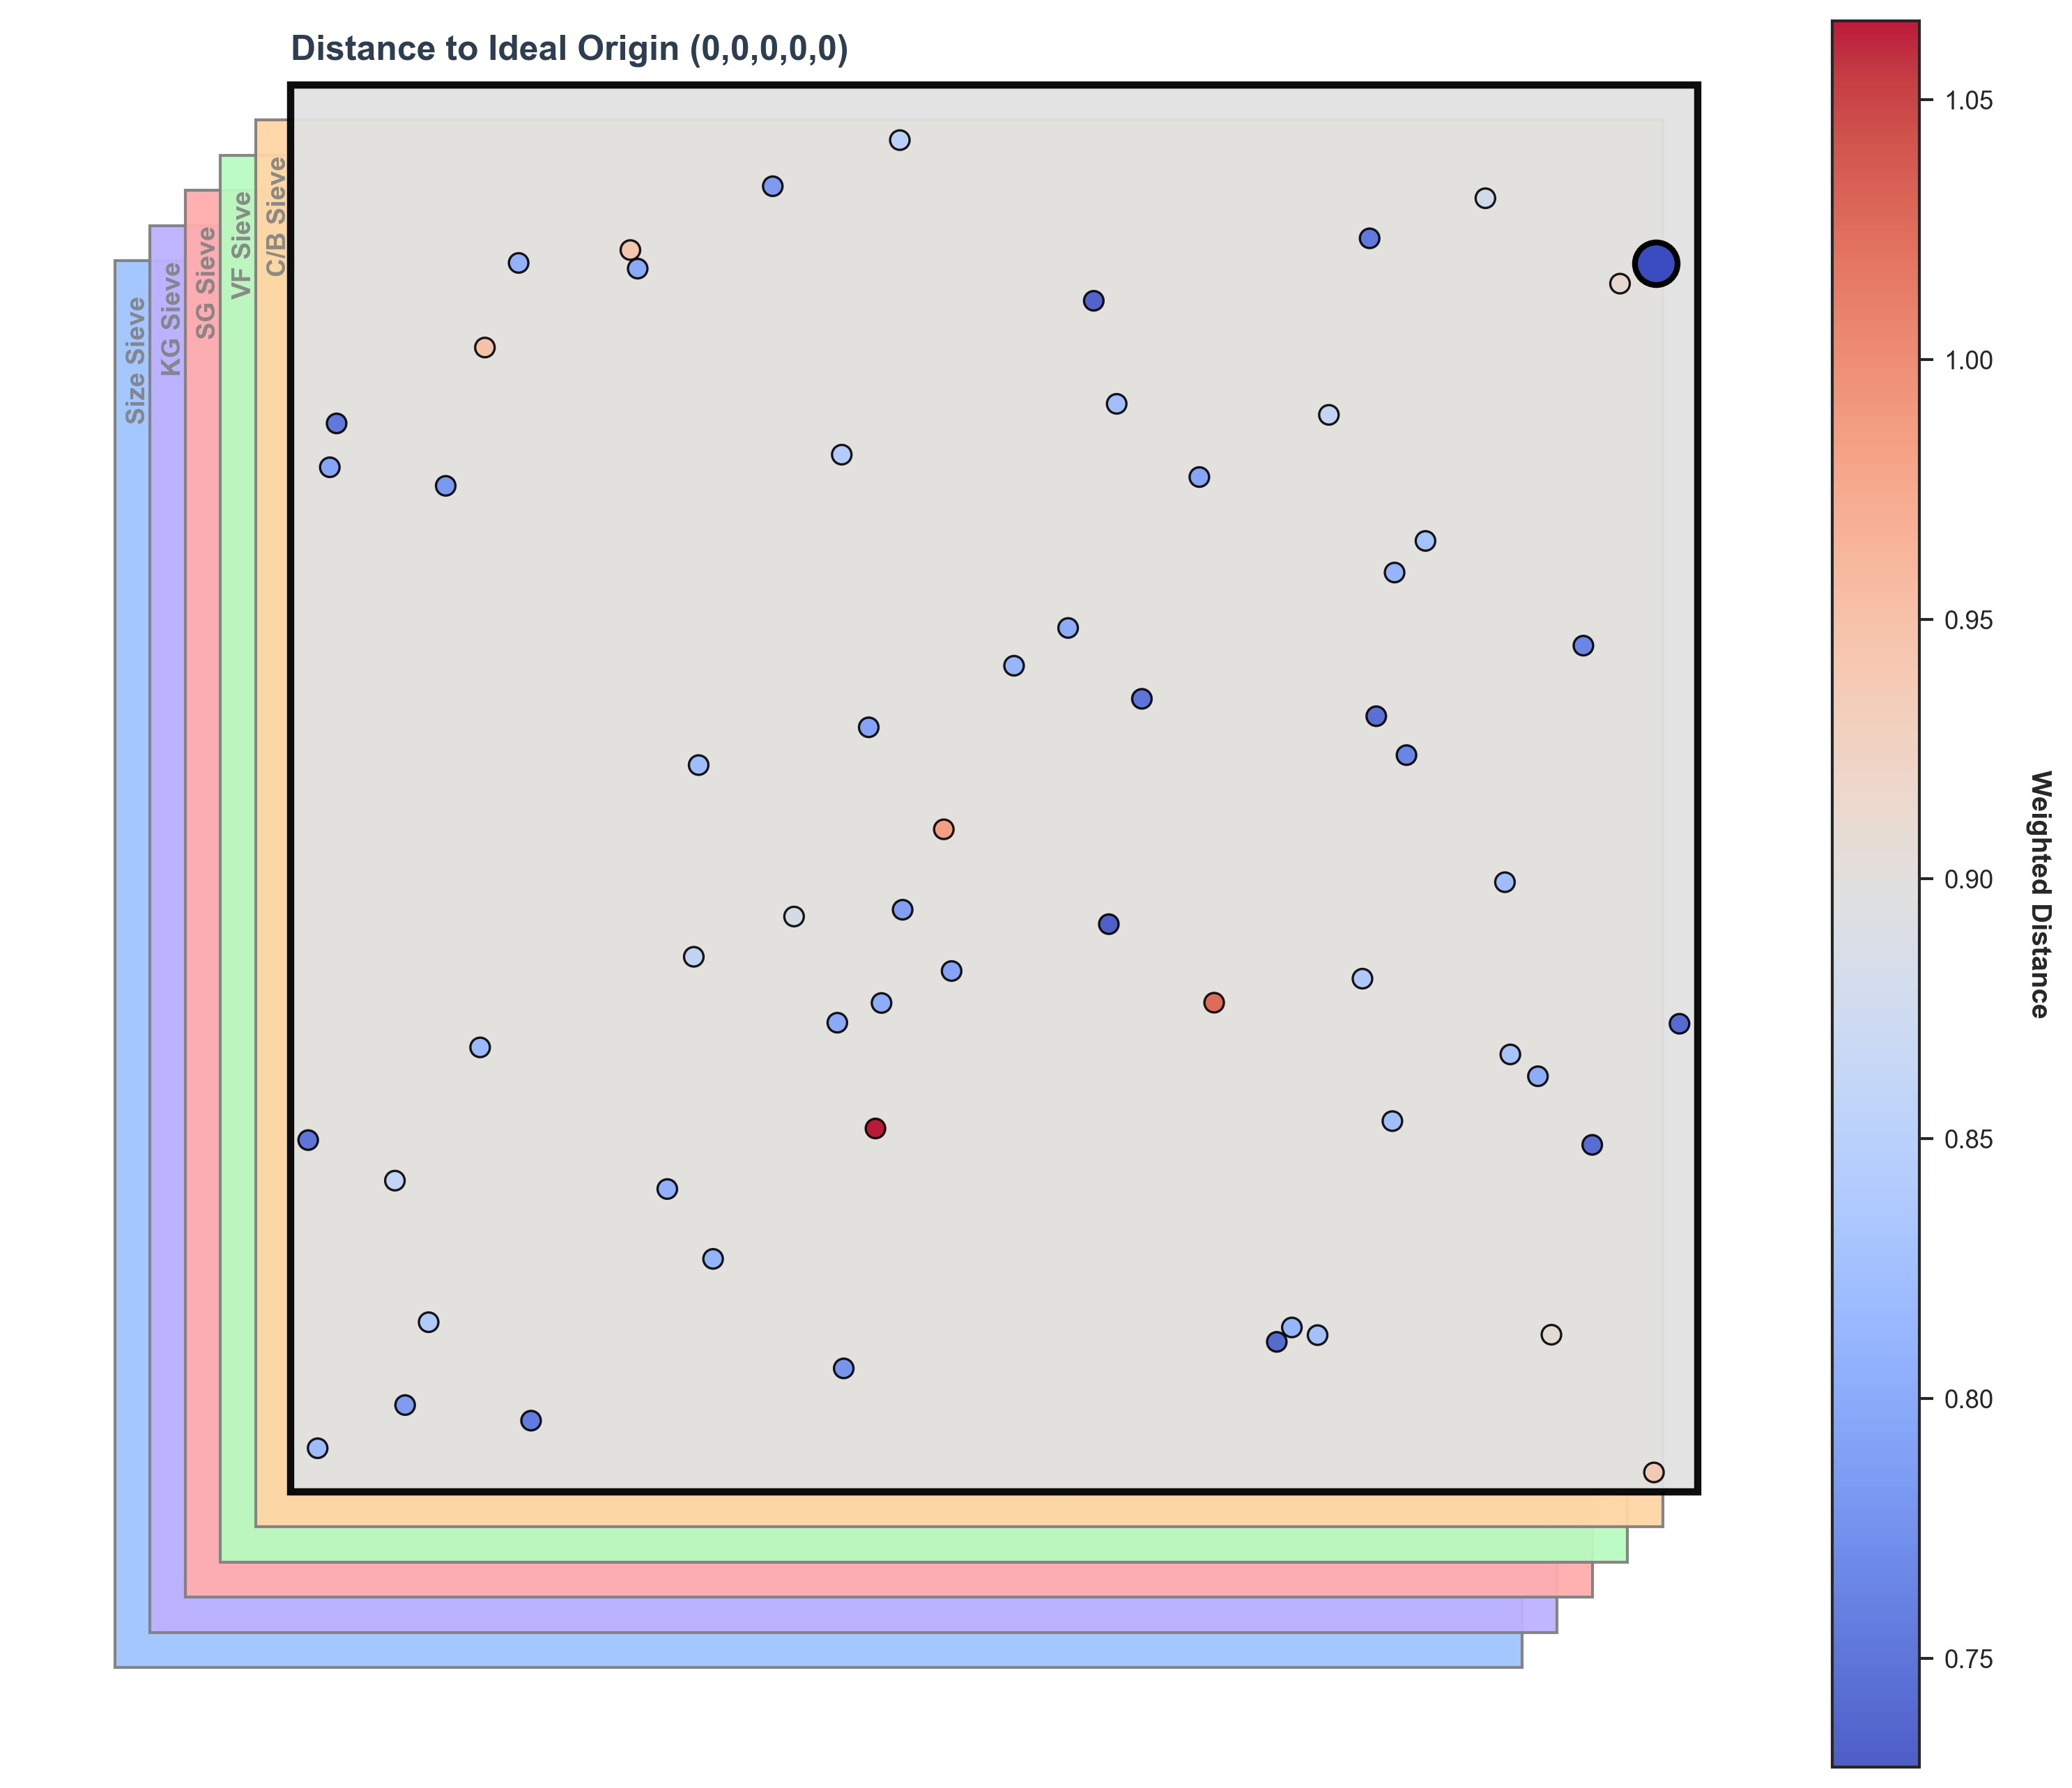
\includegraphics[width=0.75\textwidth]{content/images/sieve_step7_distance_2.png}
    \caption{Visualization of the Search for Case 2.}
    \label{fig:distance_plot_2}
\end{figure}

The resulting values are shown in Table~\ref{tab:euclidean_candidate_metrics_case_2}.

\begin{table}[htbp]
    \centering
    \small
    \caption{Performance Comparison between the Standard Baseline and the Best Shortest Distance Candidate}
    \label{tab:euclidean_candidate_metrics_case_2}
    \begin{tabular}{lrrr}
        \toprule
        \textbf{Metric} & \textbf{Standard Baseline} & \textbf{Best Candidate} & \textbf{Ratio to Std.} \\
        \midrule
        Parameters $(h, d, k, a, w)$ & $(63, 7, 14, 12, 16)$ & $(40, 5, 13, 12, 16)$ & -- \\
        Size (B) & $7,856$ & $6,160$ & $0.7841\times$ \\
        KeyGen ($C$) & $292,351$ & $146,175$ & $0.5000\times$ \\
        SigGen ($C$) & $2,218,486$ & $890,617$ & $0.4015\times$ \\
        SigVer ($C$) & $2,193$ & $1,603$ & $0.7310\times$ \\
        $\rho$ ($C$/B) & $0.2791$ & $0.2602$ & $0.9322\times$ \\
        \bottomrule
    \end{tabular}
\end{table}

Comparing the two cases, the resulting metrics differ noticeably. The first case yields more balanced costs across the board, while the second case clearly favors signature size and verification at the expense of a heavier signing operation — exactly the trade-off we asked the weights to enforce. 

\subsection{Metric-Normalized Weighted Distance} \label{sec:normalized-weights}

The weighted distance introduced in Section~\ref{sec:decisional-weights} correctly encodes relative priorities when the five ratio axes $\widetilde{X}_i$ vary over comparable ranges.
In practice, however, the filter pipeline disturbs this assumption.
Consider the signature-size filter: after it is applied with a tight coefficient $X_{\text{size}} \ll 1$, every surviving candidate has a ratio $\widetilde{X}_{\text{size}}$ that lies in a narrow band close to $X_{\text{size}}$.
The range of $\widetilde{X}_{\text{size}}$ values across survivors is therefore small relative to the variation of cost metrics such as $\widetilde{X}_{\text{kg}}$ or $\widetilde{X}_{\text{sg}}$, which the filter may leave nearly unconstrained.
As a result, the size term contributes almost the same value to $d(P)$ for every candidate in the pool, regardless of the weight $p_{\text{size}}$ attached to it.
The ranking is then dominated by the high-variance axes, and increasing $w_{\text{size}}$ produces little to no change in which candidate is selected.

The remedy is to remove the scale imbalance before applying the weights.
For each metric $i$ and each surviving candidate $P_j$ in the current pool, define the cross-pool minimum and maximum of the ratios:

\begin{equation}
    m_i = \min_j \widetilde{X}_i(P_j), \qquad
    M_i = \max_j \widetilde{X}_i(P_j).
    \label{eq:metric_range}
\end{equation}

The \emph{metric-normalized ratio} of candidate $P$ on axis $i$ is then

\begin{equation}
    \widehat{X}_i(P) = \frac{\widetilde{X}_i(P) - m_i}{M_i - m_i},
    \label{eq:metric_norm}
\end{equation}

which maps every axis to $[0, 1]$ across the survivor pool, with $\widehat{X}_i = 0$ identifying the best-performing candidate on that axis and $\widehat{X}_i = 1$ the worst-performing one.

Replacing $\widetilde{X}_i$ with $\widehat{X}_i$ in Equation~\eqref{eq:weighted_euclidean_distance} yields the \emph{metric-normalized weighted Euclidean distance}:

\begin{equation}
    d(P) = \sqrt{
        p_{\text{size}}\,\widehat{X}_{\text{size}}^2 +
        p_{\text{kg}}\,\widehat{X}_{\text{kg}}^2 +
        p_{\text{sg}}\,\widehat{X}_{\text{sg}}^2 +
        p_{\text{sv}}\,\widehat{X}_{\text{sv}}^2 +
        p_{\text{cb}}\,\widehat{X}_{\text{cb}}^2
    },
    \label{eq:normalized_weighted_distance}
\end{equation}

where the $p_i$ are the normalized weight coefficients from Equation~\eqref{eq:weight_normalization}.
The winner is still the candidate minimizing $d(P)$, but now the weight $p_i$ faithfully controls how much axis $i$ influences the ranking: because every $\widehat{X}_i$ spans the same $[0, 1]$ interval, a coefficient $p_{\text{size}} = 0.5$ means that signature size drives exactly half of the squared distance, independently of how tightly the size filter was set.
The ranges come from the current survivors, so the same weights can select a different winner after the filter changes (Appendix~\ref{app:normalization}).

Consider the following filtering parameters and weights, chosen to compare the two methods of finding the shortest vector with weights:

\begin{itemize}
    \item Filtering parameters: $X_{\text{size}} = 0.75, \ X_{\text{kg}} = 5, \ X_{\text{sg}} = 5, \ X_{\text{sv}} = 1.5, \ X_{\text{cb}} = 1$;
    \item Weight coefficients: $w_{\text{size}} = 5, \ w_{\text{kg}} = 1.5, \ w_{\text{sg}} = 1.5, \ w_{\text{sv}} = 2, \ w_{\text{cb}} = 1$.
\end{itemize}

The resulting best candidates for each method are shown in Table~\ref{tab:distance_method_comparison}.

\begin{table}[htbp]
\centering
\small
\raggedright
\caption{Comparison between the Best Candidates under the Regular Weighted and Metric-Normalized Weighted Distance Criteria}
\label{tab:distance_method_comparison}
\resizebox{\textwidth}{!}{%
\begin{tabular}{lrrrrr}
\toprule
\textbf{Metric} &
\textbf{Standard Baseline} &
\textbf{Metric-Normalized} &
\textbf{Ratio to Std.} &
\textbf{Regular Weighted} &
\textbf{Ratio to Std.} \\
\midrule
Parameters $(h, d, k, a, w)$  & $(63, 7, 14, 12, 16)$ & $(40, 4, 9, 16, 16)$  & --             & $(45, 5, 12, 11, 16)$ & --             \\
Size (B)        & $7{,}856$             & $5{,}344$             & $0.6802\times$ & $5{,}840$             & $0.7434\times$ \\
KeyGen ($C$)           & $292{,}351$           & $584{,}703$           & $2.0000\times$ & $292{,}351$           & $1.0000\times$ \\
SigGen ($C$)                  & $2{,}218{,}486$       & $4{,}108{,}285$       & $1.8518\times$ & $1{,}535{,}482$       & $0.6921\times$ \\
SigVer ($C$)             & $2{,}193$             & $1{,}308$             & $0.5964\times$ & $1{,}583$             & $0.7218\times$ \\
$\rho$ ($C$/B) & $0.2791$            & $0.2448$            & $0.8768\times$ & $0.2711$            & $0.9710\times$ \\
\bottomrule
\end{tabular}%
}
\end{table}

Comparing the two cases, the resulting metrics are different.
The regular weighted distance chooses a more balanced best candidate, while the metric-normalized weighted distance selects a candidate with a noticeably smaller signature size, trading the key and signature generation costs.

The outcome of each distance method is shown in Figure~\ref{fig:distance_result_comparison}.


\begin{figure}[h!]
    \centering
    \begin{subfigure}[b]{0.49\textwidth}
        \centering
        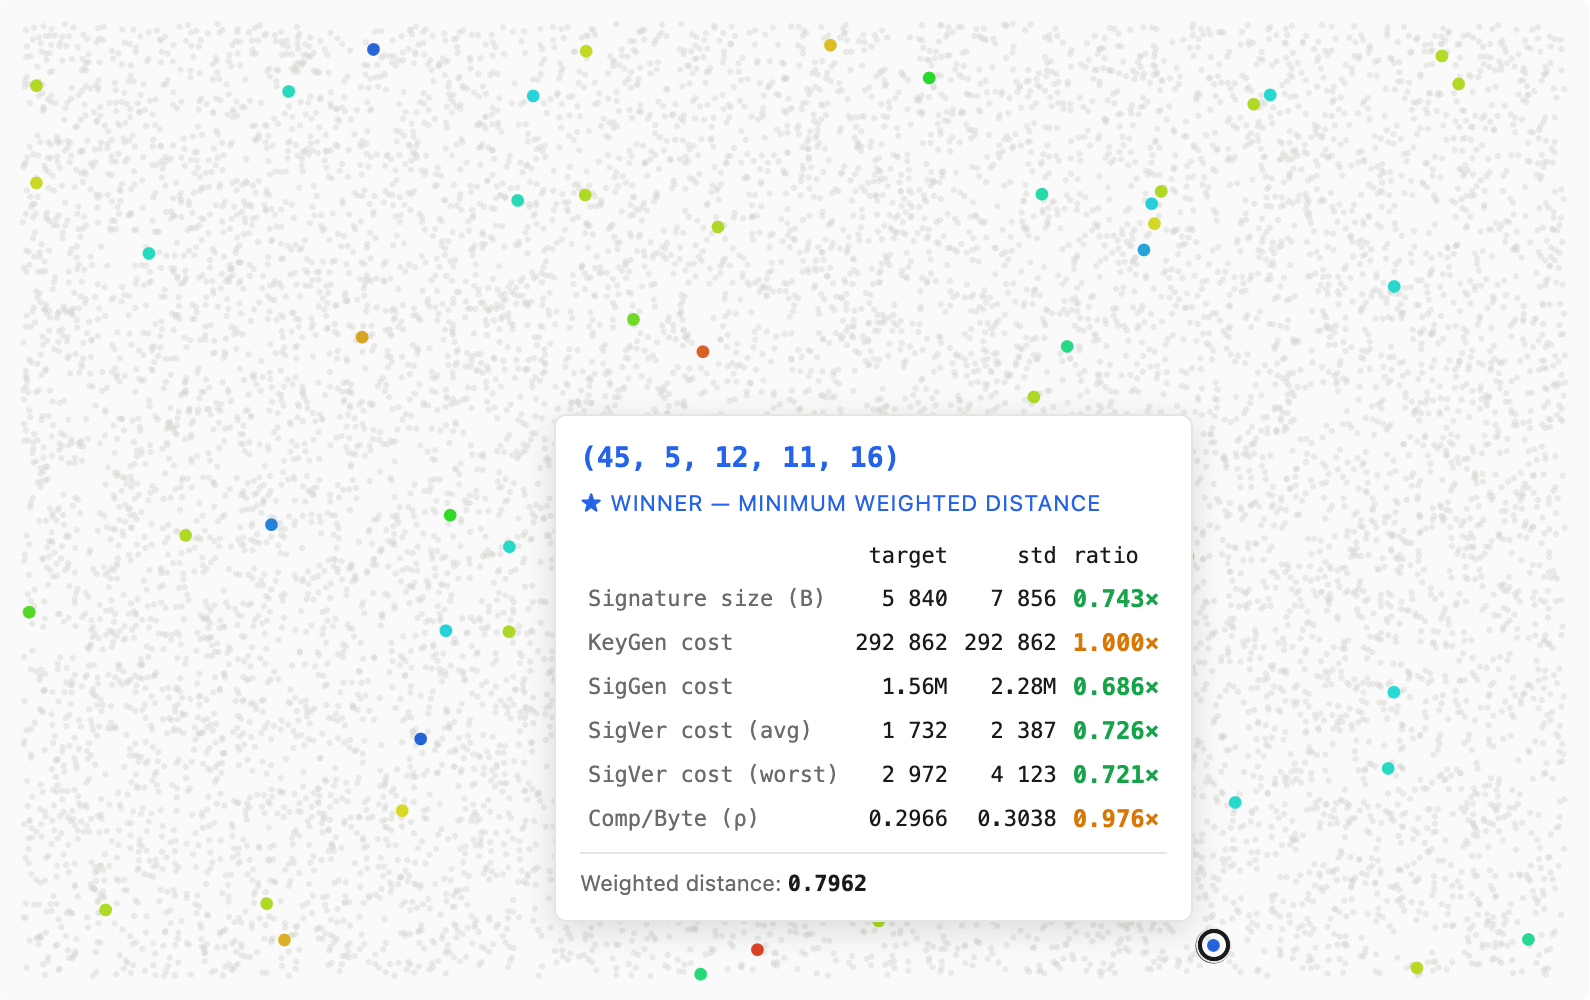
\includegraphics[width=\textwidth]{content/images/comparison_regular.png}
        \caption{Regular Weighted Distance Result}
        \label{fig:regular-weighted}
    \end{subfigure}
    \hfill
    \begin{subfigure}[b]{0.49\textwidth}
        \centering
        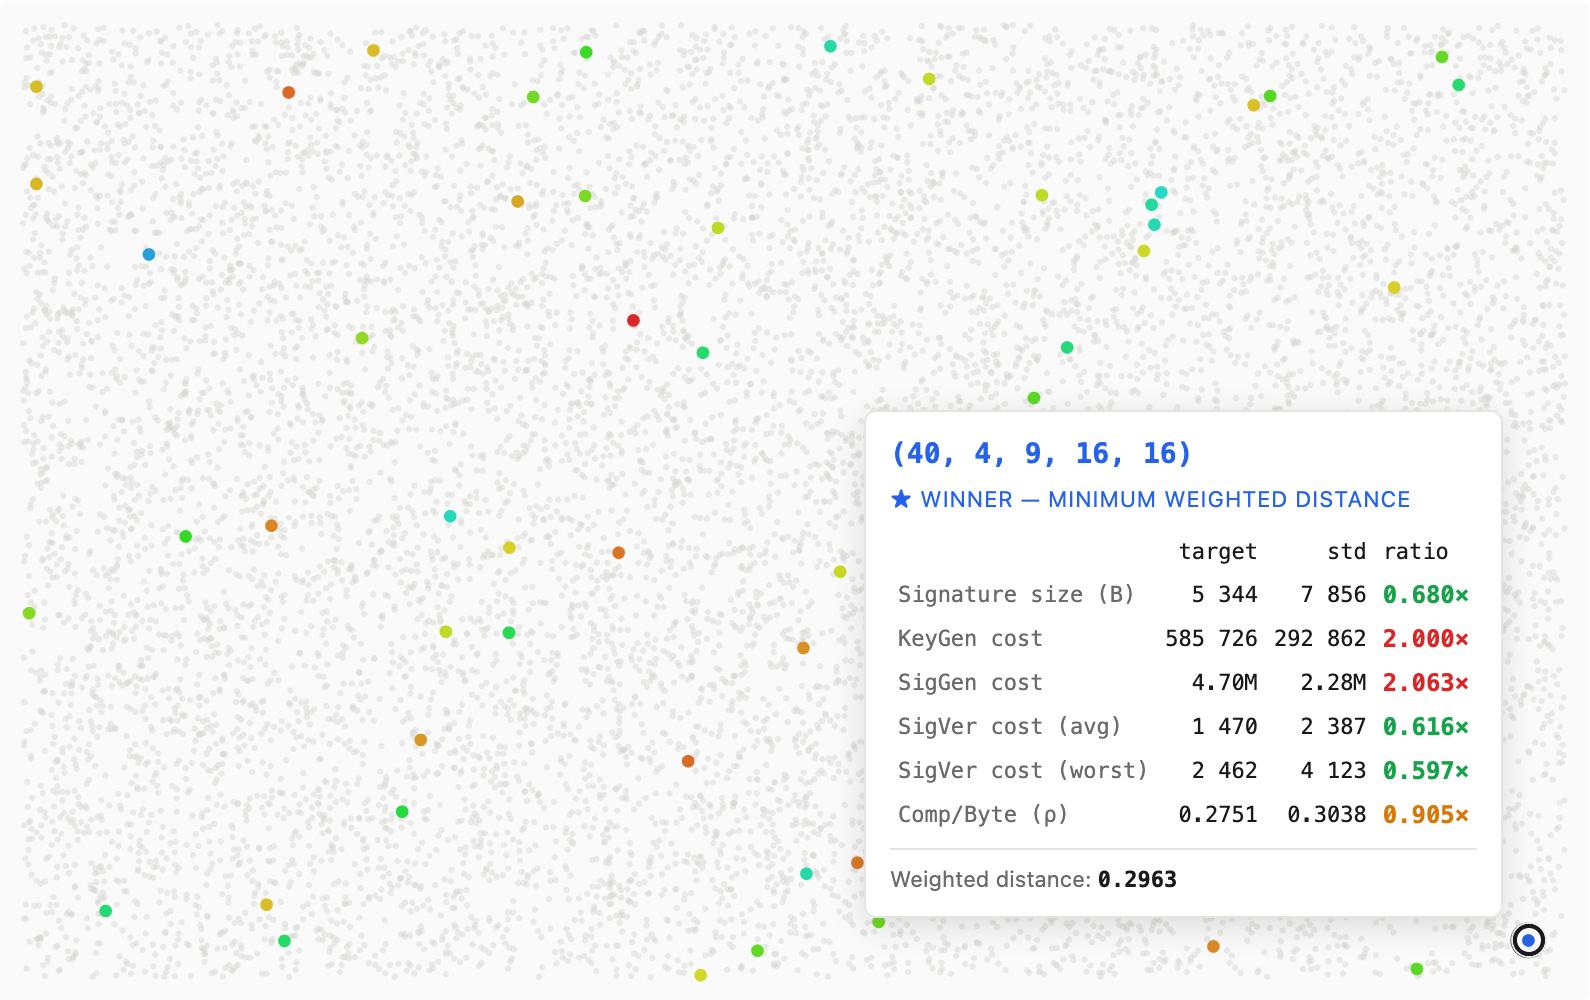
\includegraphics[width=\textwidth]{content/images/comparison_normalized.png}
        \caption{Metric-Normalized Weighted Distance Result}
        \label{fig:metric-normalised}
    \end{subfigure}
    \caption{Visualization of each Distance Method Result for Finding the Shortest Vector}
    \label{fig:distance_result_comparison}
\end{figure}
